% $Id: template.tex 11 2007-04-03 22:25:53Z jpeltier $

\documentclass{vgtc}                          % final (conference style)
%\documentclass[review]{vgtc}                 % review
%\documentclass[widereview]{vgtc}             % wide-spaced review
%\documentclass[preprint]{vgtc}               % preprint
%\documentclass[electronic]{vgtc}             % electronic version

%% Uncomment one of the lines above depending on where your paper is
%% in the conference process. ``review'' and ``widereview'' are for review
%% submission, ``preprint'' is for pre-publication, and the final version
%% doesn't use a specific qualifier. Further, ``electronic'' includes
%% hyperreferences for more convenient online viewing.

%% Please use one of the ``review'' options in combination with the
%% assigned online id (see below) ONLY if your paper uses a double blind
%% review process. Some conferences, like IEEE Vis and InfoVis, have NOT
%% in the past.

%% Figures should be in CMYK or Grey scale format, otherwise, colour 
%% shifting may occur during the printing process.

%% These three lines bring in essential packages: ``mathptmx'' for Type 1 
%% typefaces, ``graphicx'' for inclusion of EPS figures. and ``times''
%% for proper handling of the times font family.

\let\ifpdf\relax
\usepackage{mathptmx}
\usepackage{graphicx}
\usepackage{times}
\usepackage{amssymb}
\usepackage{subfig}
\usepackage{wrapfig}
\usepackage{comment}
\usepackage{epstopdf}
%% We encourage the use of mathptmx for consistent usage of times font
%% throughout the proceedings. However, if you encounter conflicts
%% with other math-related packages, you may want to disable it.

%% If you are submitting a paper to a conference for review with a double
%% blind reviewing process, please replace the value ``0'' below with your
%% OnlineID. Otherwise, you may safely leave it at ``0''.
\onlineid{0}

%% declare the category of your paper, only shown in review mode
\vgtccategory{Research}

%% allow for this line if you want the electronic option to work properly
\vgtcinsertpkg

%% In preprint mode you may define your own headline.
%\preprinttext{To appear in an IEEE VGTC sponsored conference.}

%% Paper title.

\title{MetaTracts - A Method for Robust Extraction and Visualization of Carbon Fiber Bundles in Fiber Reinforced Composites}

%% This is how authors are specified in the conference style

%% Author and Affiliation (single author).
%%\author{Roy G. Biv\thanks{e-mail: roy.g.biv@aol.com}}
%%\affiliation{\scriptsize Allied Widgets Research}

%% Author and Affiliation (multiple authors with single affiliations).
%%\author{Roy G. Biv\thanks{e-mail: roy.g.biv@aol.com} %
%%\and Ed Grimley\thanks{e-mail:ed.grimley@aol.com} %
%%\and Martha Stewart\thanks{e-mail:martha.stewart@marthastewart.com}}
%%\affiliation{\scriptsize Martha Stewart Enterprises \\ Microsoft Research}

%% Author and Affiliation (multiple authors with multiple affiliations)
\author{Arindam Bhattacharya\thanks{e-mail: arindamb86@gmail.com}\\ %
        \scriptsize The Ohio State University %
\and Christoph Heinzl\thanks{e-mail:christoph.heinzl@fh-wels.at}\\ %
     \scriptsize University of Applied Sciences - Upper Austria%
\and Rephael Wenger\thanks{e-mail:wenger@cse.ohio-state.edu}\\ %
    \scriptsize The Ohio State University}

%% A teaser figure can be included as follows, but is not recommended since
%% the space is now taken up by a full width abstract.
%\teaser{
%  \includegraphics[width=1.5in]{sample.eps}
%  \caption{Lookit! Lookit!}
%}

%% Abstract section.
\abstract{
%Carbon fiber reinforced polymers (CFRP) typically consist of two main components: the matrix and the reinforcement. 
%Most important in order to achieve the desired characteristics of a CFRP is the reinforcement component. 
%In case of CFRPs the reinforcements typically consist of bundles of endless carbon fibers woven into sheets of carbon fiber %cloth, which are then layered and combined to a CFRP by the matrix component. 
%For quality control of CFRP materials and components industrial 3D X-ray computed tomography (XCT) is increasingly applied %as it allows detailed characterizations of the material in a non-destructive manner.	

This work introduces MetaTracts, a novel method for extracting and visualizing individual fiber bundles as well as their weaving pattern in endless carbon fiber reinforced polymer (CFRP) materials, scanned by X-ray computed tomography (XCT). 

For the purpose of characterizing larger areas of CFRP materials such as complete unit cells integrating the recurring weaving pattern, the proposed workflow is designed to handle XCT scans of low resolution, in which the individual fibers of the bundles to be extracted are not or just barely visible.  
The proposed workflow applies and extends methods originally presented for the field of diffusion tensor imaging in order to cope with the low data quality: 
First, a coarse version of integral curves is used to trace subsections of the individual fiber bundles in the woven CFRP materials. We call these sections MetaTracts.
In the second step these extracted fiber bundle sections (MetaTracts) are clustered using a two step approach, wherein the first step clusters according to orientation and the second step cluster by proximity of the MetaTracts. 
Finally, the tool generates volumetric representations as well as surface models of the extracted fiber bundles to be exported for further analysis.

We evaluate the proposed workflow on a number of real world datasets and demonstrate that MetaTracts effectively and robustly identifies and separates different fiber bundles. 
%mention user study here?%
%This work will provide a stepping stone to introduce novel non destructive testing techniques for reinforced fiber bundles analysis.
} % end of abstract

%% ACM Computing Classification System (CCS). 
%% See <http://www.acm.org/class/1998/> for details.
%% The ``\CCScat'' command takes four arguments.

\CCScatlist{ 
  \CCScat{K.6.1}{Management of Computing and Information Systems}%
{Project and People Management}{Life Cycle};
  \CCScat{K.7.m}{The Computing Profession}{Miscellaneous}{Ethics}
}

%% Copyright space is enabled by default as required by guidelines.
%% It is disabled by the 'review' option or via the following command:
% \nocopyrightspace

%%%%%%%%%%%%%%%%%%%%%%%%%%%%%%%%%%%%%%%%%%%%%%%%%%%%%%%%%%%%%%%%
%%%%%%%%%%%%%%%%%%%%%% START OF THE PAPER %%%%%%%%%%%%%%%%%%%%%%
%%%%%%%%%%%%%%%%%%%%%%%%%%%%%%%%%%%%%%%%%%%%%%%%%%%%%%%%%%%%%%%%%

\begin{document}

%% The ``\maketitle'' command must be the first command after the
%% ``\begin{document}'' command. It prepares and prints the title block.

%% the only exception to this rule is the \firstsection command
%\firstsection{Introduction}

\maketitle

%\chapter {MetaTracts - Robust Extraction and Visualization of Fiber Bundles in Fiber Reinforced Composites}
%\label{metaTracts.ch}



\section{Introduction and Motivation}
\label{sec:intro}
Modern industry is increasingly demanding function orientation, integration, and efficiency of novel materials and components. The material of choice of a growing number of applications are carbon fiber reinforced polymers (CFRP), which allow an integration of those continuously rising demands in industry. CFRPs have been successfully introduced in aeronautic and automotive applications within recent years, replacing  parts made of conventional materials such as aluminum or steel. CFRP is also being used in a wide range of applications such as marine and civil engineering, automotive and wind turbine design, and also sporting goods manufacturing. 

In general, CFRP materials have desirable characteristics such as high specific stiffness, high specific strength, high corrosion resistance. CFRP materials have these characteristics  at considerably lower weight compared to conventional materials.
At the same time highly complex and integrated components which were previously  impossible to manufacture may be produced from CFRP's.
For example even primary structures and highly loaded components in aeronautics are being increasingly manufactured from CFRP.




Typically,  carbon fiber reinforced polymer components, more specifically CFRP laminates consists of two main components.
A matrix on the one side, which acts as a bonding component and  reinforcements on the other side, which allow for achieving the desired characteristics.  Various production processes are used to manufacture CFRP laminates with endless carbon fibers. Most of these processes start with the reinforcement component by weaving individual carbon fiber bundles (yarn) into sheets of carbon fiber cloth in a predefined pattern. These sheets of woven carbon fiber cloth, which form the geometrical structure of the final CFRP materials, are also referred to as fabric. Depending on the requirements of the final component as well as on the manufacturing process, fabrics may be stacked in multiple layers of the cloth. Both alignment of fabrics and the weaving pattern of the individual carbon fiber bundles strongly influence the strength, durability and stiffness properties. Resins are integrated in the material system to fill the gaps in the fabric, forming the matrix component. The main function of this matrix component is to act as a bonding component between the individual carbon fiber bundles. 
The increasing share of CFRPs and also the complexity of both material system as well as the final components generated a strong demand for non-destructive testing (NDT) techniques for quality control~\cite{Red2012}. Ultrasonic testing is the most commonly used method for non-destructive testing of carbon fiber reinforce polymers. On the one hand ultrasonic testing provides a quick and cost-efficient overview of the material. On the other hand, it shows low resolution and may generate arbitrary results, e.g. due to the geometry of the final component. 

Industrial 3D X-Ray computed tomography (XCT, also referred to as 3DXCT or cone beam XCT) is increasingly being applied for non-destructive testing of fiber reinforced polymers~\cite{Kastner2012}. XCT generates a 3D volumetric representation of the scanned specimen, reconstructed from a series of 2D penetration images, which are taken throughout a full rotation of the specimen. In industrial XCT, the typical scanning geometry places the specimen on a rotary table between X-ray source and detector. X-rays are emitted by the source in the form of a conic beam. When passing through the specimen the X-rays get attenuated by the material in the specimen. The detector records the corresponding 2D attenuation image (penetration image) by transferring the X-rays in a scintillator layer into visible light. To generate the required series of 2D penetration images of a full $360^\circ$ rotation for a complete reconstruction of the data volume, the specimen is rotated stepwise and at each position a cone beam penetration image is recorded~\cite{heinzl-2008-thesis}. Finally the series of penetration images is  reconstructed as a 3D volumetric dataset of the specimen. 
In state of the art devices, XCT can reach voxel sizes below $500 nm$. XCT generates high resolution volume data for comprehensive and detailed analyses of the test specimens. Unfortunately, there is still a trade-off between viewport and image resolution in XCT using cone beam geometry. The magnification reached within an XCT scan is determined by the specified distances between source and specimen as well as source and detector. The magnification therefore directly influences both resolution and viewport: higher resolutions decrease the viewport but show more details while lower resolutions allow for larger viewports and thus larger portions of the specimen.

In this work, we focus on datasets with larger viewports and lower resolutions where the single carbon fibers (filaments) are not or are  barely visible. Our domain experts are mainly interested in visualizing the geometric structures in the weaving pattern of fiber bundles in endless carbon fiber reinforced composites instead of high resolution studies of  individual fibers.
%of short fiber reinforced composites as presented by Weissenbock2014 et al.~\cite{Weissenbock2014}.
Figure~\ref{fig:data-char} provides an example of our targeted datasets. It also shows the recurring fiber bundle pattern in the final CFRP laminate, called a \textit{unit cell}.
Our work is motivated from the recent progress in two interrelated fields: On the one hand, CFRP components have gained wide application in a variety of industries  because of its superior material and physical properties in comparison to conventional materials \cite{Karpat2012}. On the other hand, recent developments of industrial 3D X-Ray computed tomography (XCT) with regard to larger detectors, larger field of views and better resolutions opened XCT for this new application area of non destructive testing for fiber reinforced components~\cite{Schilling2005}. 

% Fiber bundles determine to a large extent the properties in terms of specific stiffness, specific strength, or durability of the final component. However, when scanning reinforced polymers using modern XCT devices, there is still a trade-off between view port and image resolution. Due to the intrinsic concept of cone beam and fan beam XCT setups, the magnification reached within a scan is determined by the used distances between source and specimen as well as source and detector. Furthermore the magnification directly influences both resolution and viewport: Higher resolutions decrease the viewport or how much of the structure can be imaged while lower resolutions allow for larger view ports.
%\begin{figure}
%\begin{center}
%\includegraphics[width=0.3\textwidth]{imagesMetaTracts/crop-13-total}
%\caption{Volume rendering of a part of a dataset. Fig~\ref{fig:slice_data:a} and ~\ref{fig:slice_data:b} show image slices along the blue and red plane respectively.  }\label{fig:orig_data}
%\end{center}
%\end{figure}
%!!!!! TODO REFINE DTI PARAGRAPH !!!!!
%Diffusion Tensor Imaging tractography clustering and visualization.
%The topic of DTI visualization has seen an extensive amount of investigation by researchers.
%Advantage of two phase clustering 
%What is the  motivation for fiber-lets
%Seed point selection 
%distance between tracks 
%how well do we do in noise , may be data set 1

%!!!!! I have replaced this with the following para !!!!!
%In this work, we present a framework which interprets and advances these techniques in order to extract and visualize fiber bundles in industrial 3D X-Ray computed tomography data of woven fiber reinforced composites. The main goal of this work is to expand the state of the art in nondestructive testing of composite structures towards lower resolutions and thus larger areas of woven fabrics.

%While the importance of fiber bundles in determining the final properties of the components have  become evident,  the tools for visualization of the same have not developed at the same pace.

While fiber bundles are now understood as highly important in determining component properties, the tools for visualization of the internal structure have not developed at the same pace.
To the best of our knowledge, there is no current work that can resolve simple queries such as:
\begin{itemize}
\item{ How to extract and visualize the geometric structure of a particular fiber bundle?}
\item{ How to visualize the interaction between a particular pair of fiber bundles (crossovers/braiding) or a unit cell?}
\item{ Which fiber bundles show a particular orientation? }
\item{ Which fiber bundles are of the same type of yarn (i.e. which bundles show similar sizes or diameters), which is the largest or smallest fiber bundle?}
\end{itemize}

Answering the above queries from the volume renderings of XCT datasets, or from visual inspection of particular 2D slices is non-trivial, even for experts. We detail and evaluate a method which uses visualization techniques to gain insight into our data. We demarcate the above queries into two parts, ``geometric structure" and ``spatial context". Geometric structure refers to the shape, size, and orientation of a fiber bundle or a group of bundles. Spatial context refers to how two or more bundles interact with each other. 
We advance and interpret techniques from diffusion tensor imaging to extract and visualize geometric structures from 3D X-Ray computed tomography data of the woven carbon fiber reinforced composites. The main goal of this work is to expand the state of the art in non-destructive testing through visualization of composite structures in ``lower resolutions" and thus ``larger areas" of woven fabrics.

The paper is structured as follows: Section~\ref{sec:prev_work} reviews the related work,  Section \ref{sec:char_data} describes the   characteristics of our data. Sections \ref{sec:approach},~\ref{subsec:fiber-bundles},~\ref{sec:vis} provides details of our approach. Section \ref{sec:results} details experiments, section~\ref{sec:user_eval} summarizes our user evaluation results. Section~\ref{sec:param_choices} explains our  parameter choices. We end with conclusions in section~\ref{sec:conclusions}.



\section {Related work}
\label{sec:prev_work}
%In order to analyze fiber bundles, whose individual fibers are barely visible, we studied a branch of visualization which seems to be completely off-topic at first sight: Diffusion Tensor Imaging (DTI). Tractography methods to reconstruct fibrous structures such as neural fibers in the human brain from magnetic resonance (MR) images has seen extensive research in recent years. Visualization techniques to reduce the geometric complexity and cluttering caused by dense fiber models of single fibers and emphasizing higher level structures called the fiber bundles have also gained popularity in recent years. In general these bundles are related anatomically or spatially.
%We broadly divide the related work on DTI  into two parts related to our method: fiber tracking and fiber clustering. Furthermore, methods analyzing second order local structure are considered as related work. Finally, we review the field of visual analysis of fiber reinforced composites in this section.

Diffusion Magnetic Resonance Imagining (dMRI, also referred to as Diffusion Tensor Imaging (DTI)) has gained popularity in medical diagnosis within recent years. Its main clinical application is found in the study and treatment of neurological disorders. DTI may reveal abnormalities in white matter fiber structure and is used for visualizing the organization of white fibers in the human brain and  brain connectivity.
A variety of algorithms have been proposed aiming for generating fiber-tract trajectories. In general, these reconstructions of fiber trajectories are  clustered in bundles which are expected to be related anatomically or spatially. 
We broadly divide the related work on DTI into two parts that are of immediate relevance to our proposed solution: fiber tracking and fiber clustering. We discuss  methods for analyzing the second order local structure. Finally, we review the current state of the art in the visual analysis of fiber reinforced composites.


\subsection {Fiber Tracking in Diffusion Tensor Imaging}
\label{subsec:fiberEx} 
A basic assumption in DTI analysis is that the principal eigenvector of the diffusion tensor is parallel to the underlying dominant fiber direction in each image voxel~\cite{Basser2002, Basser2000, Mori1999, Mori2002}. Continuous tracts are created by propagating virtual particles along fiber directions until they reach some termination criterion. 
 This is usually done by solving a second-order Runge-Kutta integration. The principal diffusion direction at each discrete location is interpolated to from a continuous velocity field. 
 Because decisions are made locally, these methods perform poorly in noisy regions and often generate small fibers. Basser et al.~\cite{Basser2000},~\cite{Basser2002} proposed that white matter tracts could be represented as 3D curves in space. They showed that numerical methods could be used to follow fibers and fiber bundles and to generate tracts in human brain data. 
Mori et al.~\cite{Mori1999},~\cite{Mori2002} showed that tract reconstruction techniques could be broadly divided into line-propagation or energy minimization techniques. In line propagation approaches, trajectories are computed based on local neighborhoods and in energy minimization approaches the most  favorable trajectory connecting two given endpoints is selected. 


\subsection {Fiber Clustering in Diffusion Tensor Imaging}
\label {subsec:fiberClus}
In DTI, a similarity measure based on factors such as proximity between fibers is used to group fiber tracts into bundles. Extensive research has been done on automatic DTI fiber clustering methods~ \cite{Corouge2004, Brun2003, Brun2004, Zhang2008, westinMEDIA02}. 
Clustering requires choosing a suitable proximity measure and choosing a method for grouping ``close" fibers.
Pairwise proximity measures include endpoint distances~\cite{Brun2003} and mean of the closest distances between points on two fibers~\cite{Corouge2004}. Zhang et al.~\cite{Zhang2008} introduced a thresholded version of the of mean of closest distances, so that fibers that are close for certain distance and then diverge are clustered separately. Brun et al.~\cite{Brun2004} uses normalized cuts along with a pairwise distances  measure computed using a 9-D fiber shape descriptors. The choice of the clustering algorithm can be broadly divided into those approaches using hierarchical clustering ~\cite{Moberts2005, Zhang2008} and those using spectral clustering ~\cite{jonasson2005, ODonnell2007, Brun2004}.
 
Brun et al.~\cite{Brun2003} described how a spectral non-linear dimensionality reduction technique,  Laplacian eigenmaps (Belkin and Niyogi~\cite{Belkin01}) can be applied to the problem of organizing fiber trace data. The key notion of the Laplacian eigenmaps algorithm is to represent the underlying data as a graph. Each node represents a data point and the edges connect neighboring data points. An eigenvalue problem is solved to represent the data in a lower dimensional space while preserving the local graph structure. In the case of fiber bundles, the individual points are fiber traces. In the ideal case fiber traces that belong to the same bundle must remain ``close" to each other in the lower dimensional space. Westin et al.~\cite{westinMEDIA02} also use spectral clustering on a Hausdorff distance measure defined as the maximum of pointwise minimum distances between two fibers. Jonasson et al.~\cite{jonasson2005} run k-means clustering on the eigenvectors of the affinity matrix defined as the co-occurrence of fibers in the data.
%The clustering methods have also been evaluated to be generally accurate in capturing fiber bundles as seen in Moberts et al.~\cite{Moberts2005} and Corouge et al.~\cite{Corouge2004}. 

The agglomerative hierarchical clustering method \cite{DudaHartStork01} has gained popularity for proximity based fiber segregation Zhang et al.~\cite{Zhang2008}, Corouge et al.~\cite{Corouge2004}. 
These approaches build on the assumption that proximity measures that compare DTI fiber trajectories can also represent anatomical relationship. An agglomerative hierarchical clustering method starts with each data point/fiber in an individual cluster. At each stage of the algorithm the two most similar clusters are joined. The two basic cluster similarity measures are single-link and complete-link. With the single link measure the distance between the clusters is the distance between the closest pair of items. 
Moberts et al.~\cite{Moberts2005} implemented several distance measures in their evaluation of fiber clustering and concluded that clustering methods are generally accurate in capturing fiber bundles. 
%Mean of closest distances performs better than closest point distance computations or Hausdorff distance measures and hierarchical clustering using single-link measure gave the best results. 

There are a number of difficulties in hierarchical clustering. First, computing all pairs distances for tracts to generate the distance matrix is time consuming (see~\cite{Garyfallidis2012} for a recent work on decreasing computation times). Second, a ``correct'' distance measure to compare tracts must be chosen. Thirdly, hierarchical clustering is best suited for similar length fibers.
Spectral methods are also hindered by long matrix computations.


\subsection{Second order local structure}
%!!!!! TODO REFINE SECTION !!!!!
Unlike DTI, we do not have diffusion tensor data. Instead, we have a scalar volume with tubular structures embedded in them. Analyzing curvilinear structures in volumetric images has been utilized for a variety of purposes including center line extraction~\cite{Bouix2005} and vascular image enhancement as proposed by Frangi et al.~\cite{Frangi1998} and Sato et al.~\cite{Sato1997}. Frangi et al.~\cite{Frangi1998} introduced a method based on studying the eigenvalues of the  Hessian matrix specifically for the purposes of developing vessel enhancement filters.


\subsection {Visual Analysis of Fiber Reinforced Composites}
The approaches presented in visualization and analysis of composites mainly focus on individual objects such as fibers or pores: Fritz et al.~\cite{Fritz2009} proposed interactive workflows for non destructive testing practitioners to explore and quantify steel fibers in reinforced sprayed concrete. This approach allows analyzing fiber orientations based on direction transfer functions. Salaberger et al.~\cite{Salaberger2011} introduced a pipeline to extract and characterize individual fibers of fiber reinforced composites. They encode the extracted fibers as color-coded line segments in 3D and visually identifying fibers with similar orientations. Reh et al.~\cite{PMI_AR_2012} introduced an approach to explore pores of carbon fiber reinforced composites. Recently, Weissenbock et al.~\cite{Weissenbock2014} introduced a system for interactive exploration and analysis of fibers in fiber reinforced polymers. 

Tools based on image analysis, fiber tracking and clustering into bundles in DTI and their subsequent visualization through stream tubes and coloring schemes has received extensive research and recently the application of similar techniques to fiber tracing in composite materials has gained momentum. To the best of our knowledge there is no approach focusing on direct extraction of fiber bundle structures from low resolution XCT of composite fibers, which is the main scope of this work.

%To the best of our knowledge there is no approach focusing extraction of fiber bundles structures of low resolution XCT  of composite fibers, which is the main scope of this work.

%\begin{figure}
%  \begin{center}
%    \includegraphics[width=0.25\textwidth,clip=true, trim=2cm 2cm 0cm 2cm]{imagesMetaTracts/crop-13-total}
%  \end{center}
% \caption{Volume rendering of a part of a dataset. Fig.~\ref{fig:slice_data:a} and ~\ref{fig:slice_data:b} show image slices along the blue and red plane respectively. }
% \label{fig:orig_data}
%\end{figure}
%\begin{figure}[h]
%  \centering
%              \subfloat [][A single slice along blue plane in fig~\ref{fig:orig_data}.]
%                        {\includegraphics[width=0.22\textwidth]{imagesMetaTracts/crop-13-1c-anno.png}\label{fig:slice_data:a}}\quad 
%                        \subfloat [][A single slice along the red plane in fig~\ref{fig:orig_data}]
%                        {\includegraphics[width=0.22\textwidth]{{imagesMetaTracts/crop-13-1b-anno}}\label{fig:slice_data:b}}
%  \caption{Single slices along different orientations of the data set. In Fig.~\ref{fig:slice_data:b}, the red annotation demarcates the boundary between two different bundles. The green squares show that the cross sections of the bundles also widely vary.}
%  \label{fig:slice_data}
%\end{figure}

\begin{figure}[tb]
\centering
%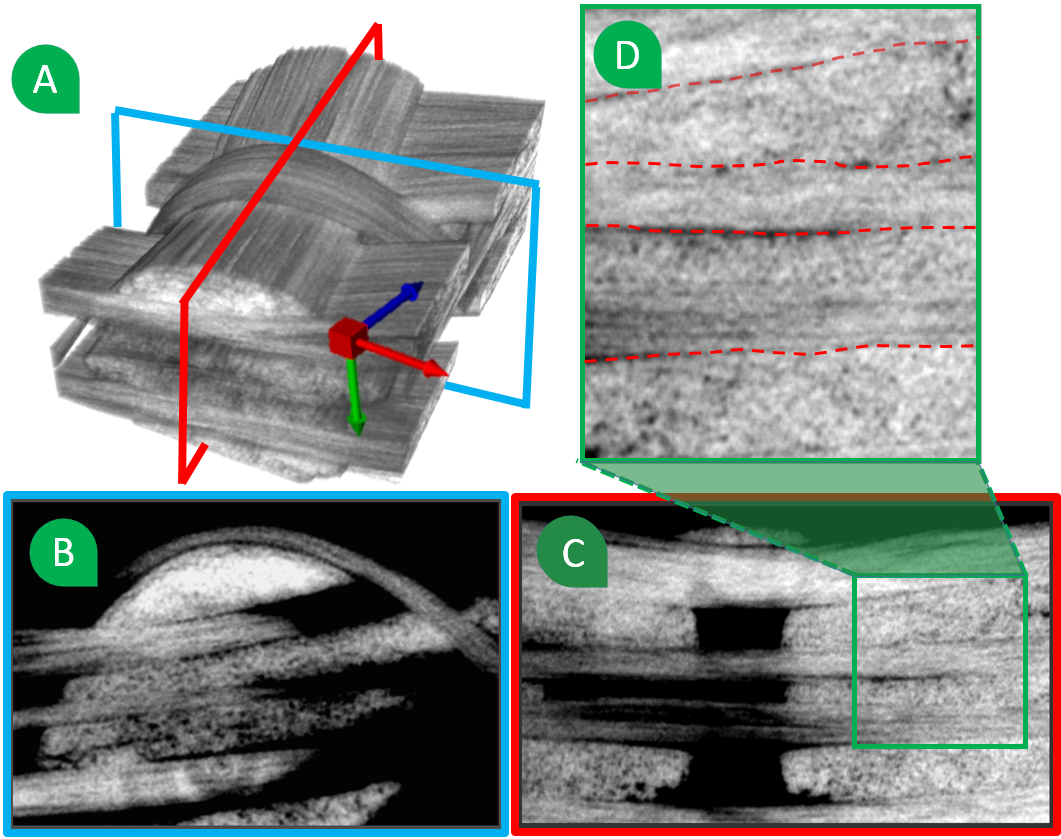
\includegraphics[width=0.45\textwidth]{imagesMT2014/MT_data_4_2.png}
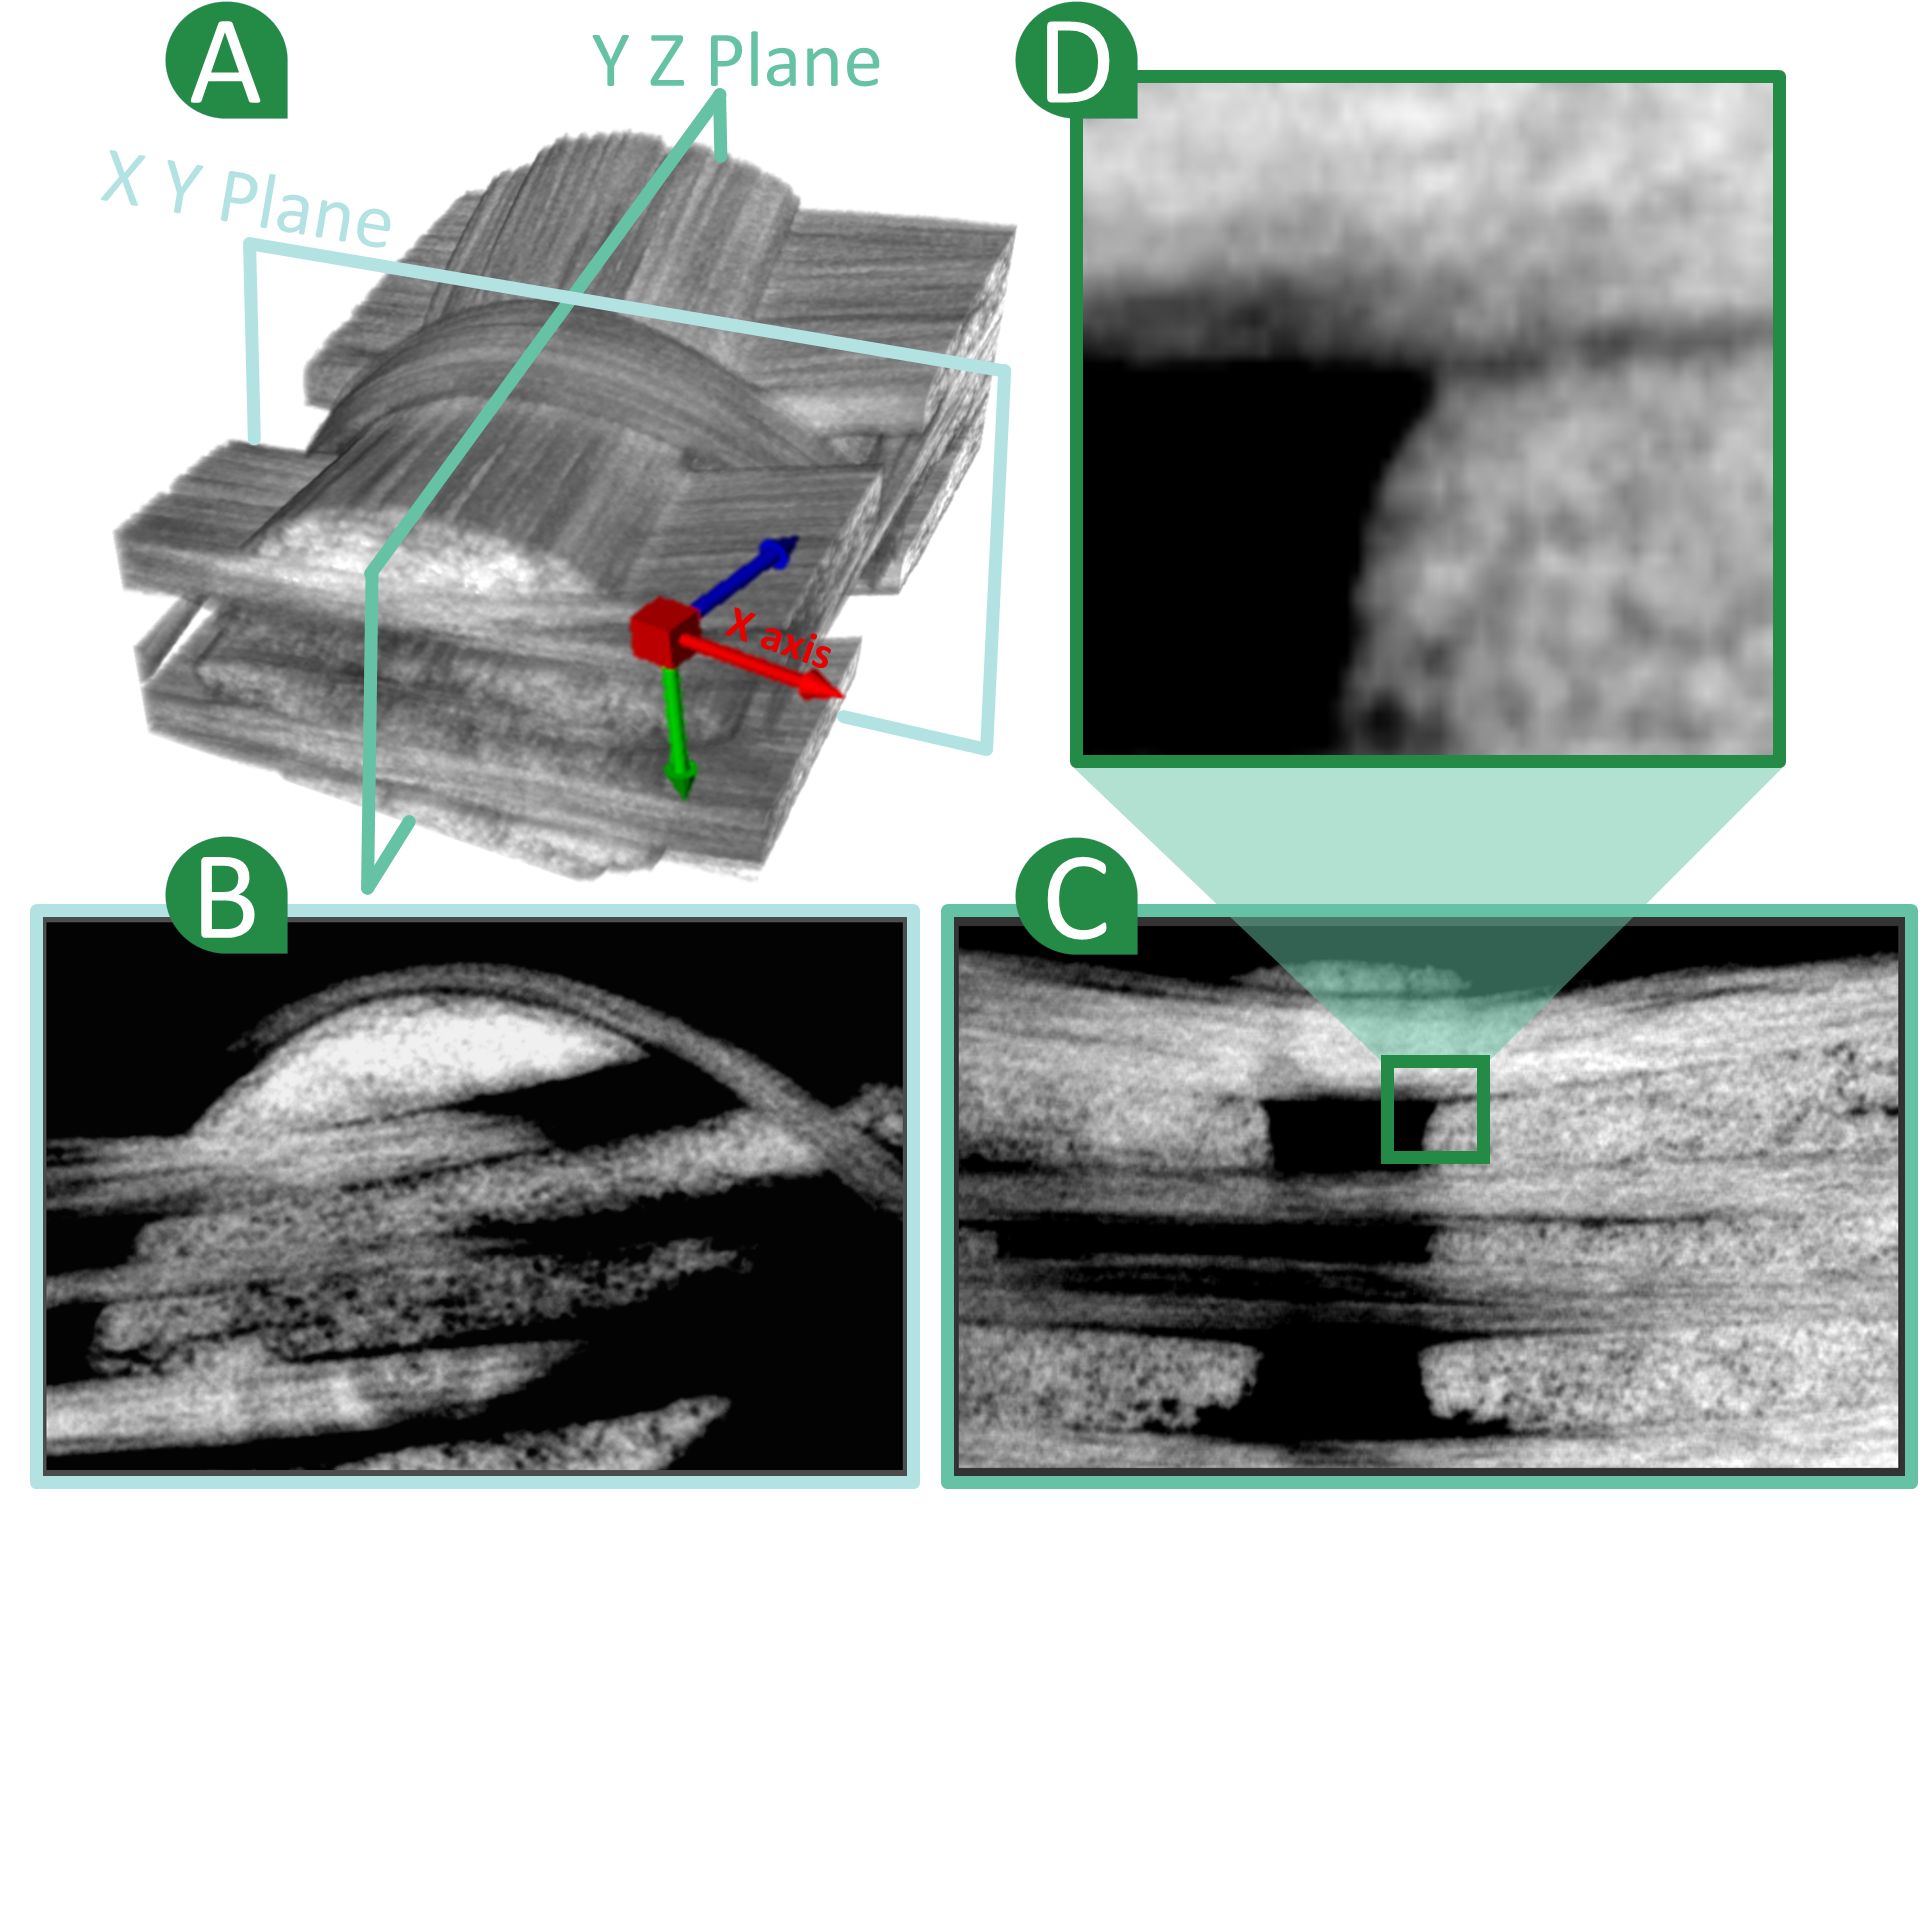
\includegraphics[width=0.5\textwidth, trim = 0mm 110mm 0mm 0mm, clip,]{images_pvis/figure1}
\caption{Data Characteristics. (A) shows a rendering of the data. (B) shows 2D slices along the X and (C) along the Z axis. (D) close up of the region marked in green in (C), multiple fiber bundles cross and are indistinguishable by visual inspection alone. }
\label{fig:data-char}
\end{figure}
\section {Data Characteristic and Assumptions}
\label{sec:char_data}

Figure \ref{fig:data-char} shows dataset1 with woven fiber bundles. Dataset1 is 450x300x500 voxels in size with isotropic resolution of $2\mu m$, the data type is unsigned 8 bit integer. Fig.~\ref{fig:data-char} clearly shows the weaving structure of the composite unit cell as regional subset of the recurring fiber bundle weaving pattern. The unit cell is used as a basis structure for CFRP manufacturing. The alignment and weaving pattern of the fiber bundles in the cloth influences the strength and stiffness properties of the resulting material. Figure~\ref{fig:data-char}(A) shows a volume rendering of the dataset. Fig.~\ref{fig:data-char}(B) shows 2D slices along the X and Fig.~\ref{fig:data-char}(C) in Z(left) axis. Figure~\ref{fig:data-char}(D) shows the magnified version of the green square. 
The resolution of dataset1 renders the individual carbon fibers in a fiber bundle are hard to resolve using 2D slice images only. Figure~\ref{fig:data-char}(D) contains two bundles going in opposite directions. However, the separation between two fiber bundles is barely visible. The carbon fibers themselves do not differ much from the underlying epoxy matrix in terms of attenuation which poses an additional challenge for characterization. The fiber bundles themselves may differ in terms of the amount of fibers in the bundle. Figure~\ref{fig:data-char}(A) shows the large variation in cross section sizes among the bundles.
Depending on the weaving pattern the fiber bundles cross each other in different orientations. In general the number of orientations is limited by the weaving pattern. In all our data sets the number of separate orientations was two. Nevertheless, the weaving pattern may cause the individual bundles to be curved. In consequence of the weaving pattern of the fiber bundles, individual fibers may be adjacent in Euclidean distance but belong to different bundles. 
We make the following assumptions on our data:
\begin{itemize}
\item The structure embedded in the data contains fiber bundles of indiscernible fibers.
\item (Local orientation) Each point within a fiber bundle has a local orientation which is parallel to the corresponding area in the fiber bundle.
\item The local orientation may change gradually inside the fiber bundle.
\item The local orientation may be noisy and not reliable.
\item (Connectivity) Moving along the direction of a non-noisy local orientation in small increments, we will reach another neighborhood with similar local orientation.
\item Fiber bundles going in different directions only interact near the surface of contact.
\end{itemize}
%\begin{figure}[htp]
%  \centering
%    \subfloat[Overview of the dataset]{\label{figur:3}\includegraphics[scale=0.3]{imagesMetaTracts/crop13-a.eps}}
%  \subfloat[X Axis]{\includegraphics[width=40mm, height=40mm]{imagesMetaTracts/xaxis.eps}}\label{figur:1}\\
%  \subfloat[Y Axis]{\label{figur:2}\includegraphics[width=40mm, height=40mm]{imagesMetaTracts/yaxis.eps}}
%  \subfloat[Z Axis]{\label{figur:3}\includegraphics[width=40mm, height=40mm]{imagesMetaTracts/zaxis.eps}}
%  \caption{One of our datasets.Fig \ref{fig:orig_data}(a) provides an overview of the entire volume, the rest show slices of each of the major axis.}\label{fig:orig_data}
%\end{figure}

%\begin{figure}[b]
%\centering
%\includegraphics[width=\linewidth]{imagesMetaTracts/crop-13-3.eps}
%\caption{Volume rendering of the scalar volume of one of our data set. Cut-out A shows a slice along the X axis, cut-out B shows a slice along the Z axis.}\label{fig:orig_data}
%\end{figure}


\section {Extracting MetaTracts }
\label{sec:approach}

\begin{figure}[t]
	\centering
%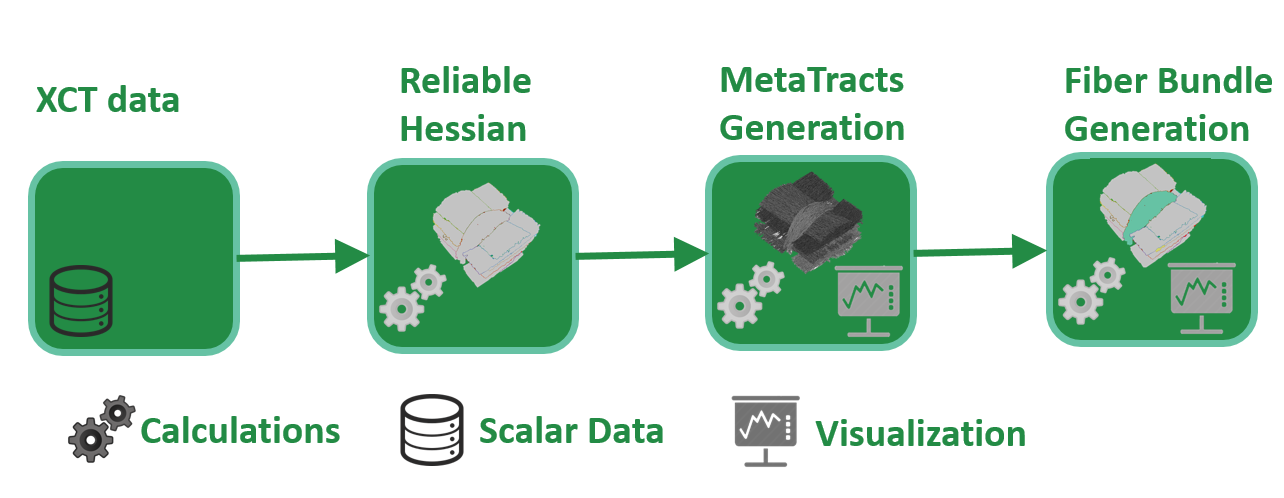
\includegraphics[width=0.45\textwidth]{imagesMT2014/algo.png}
%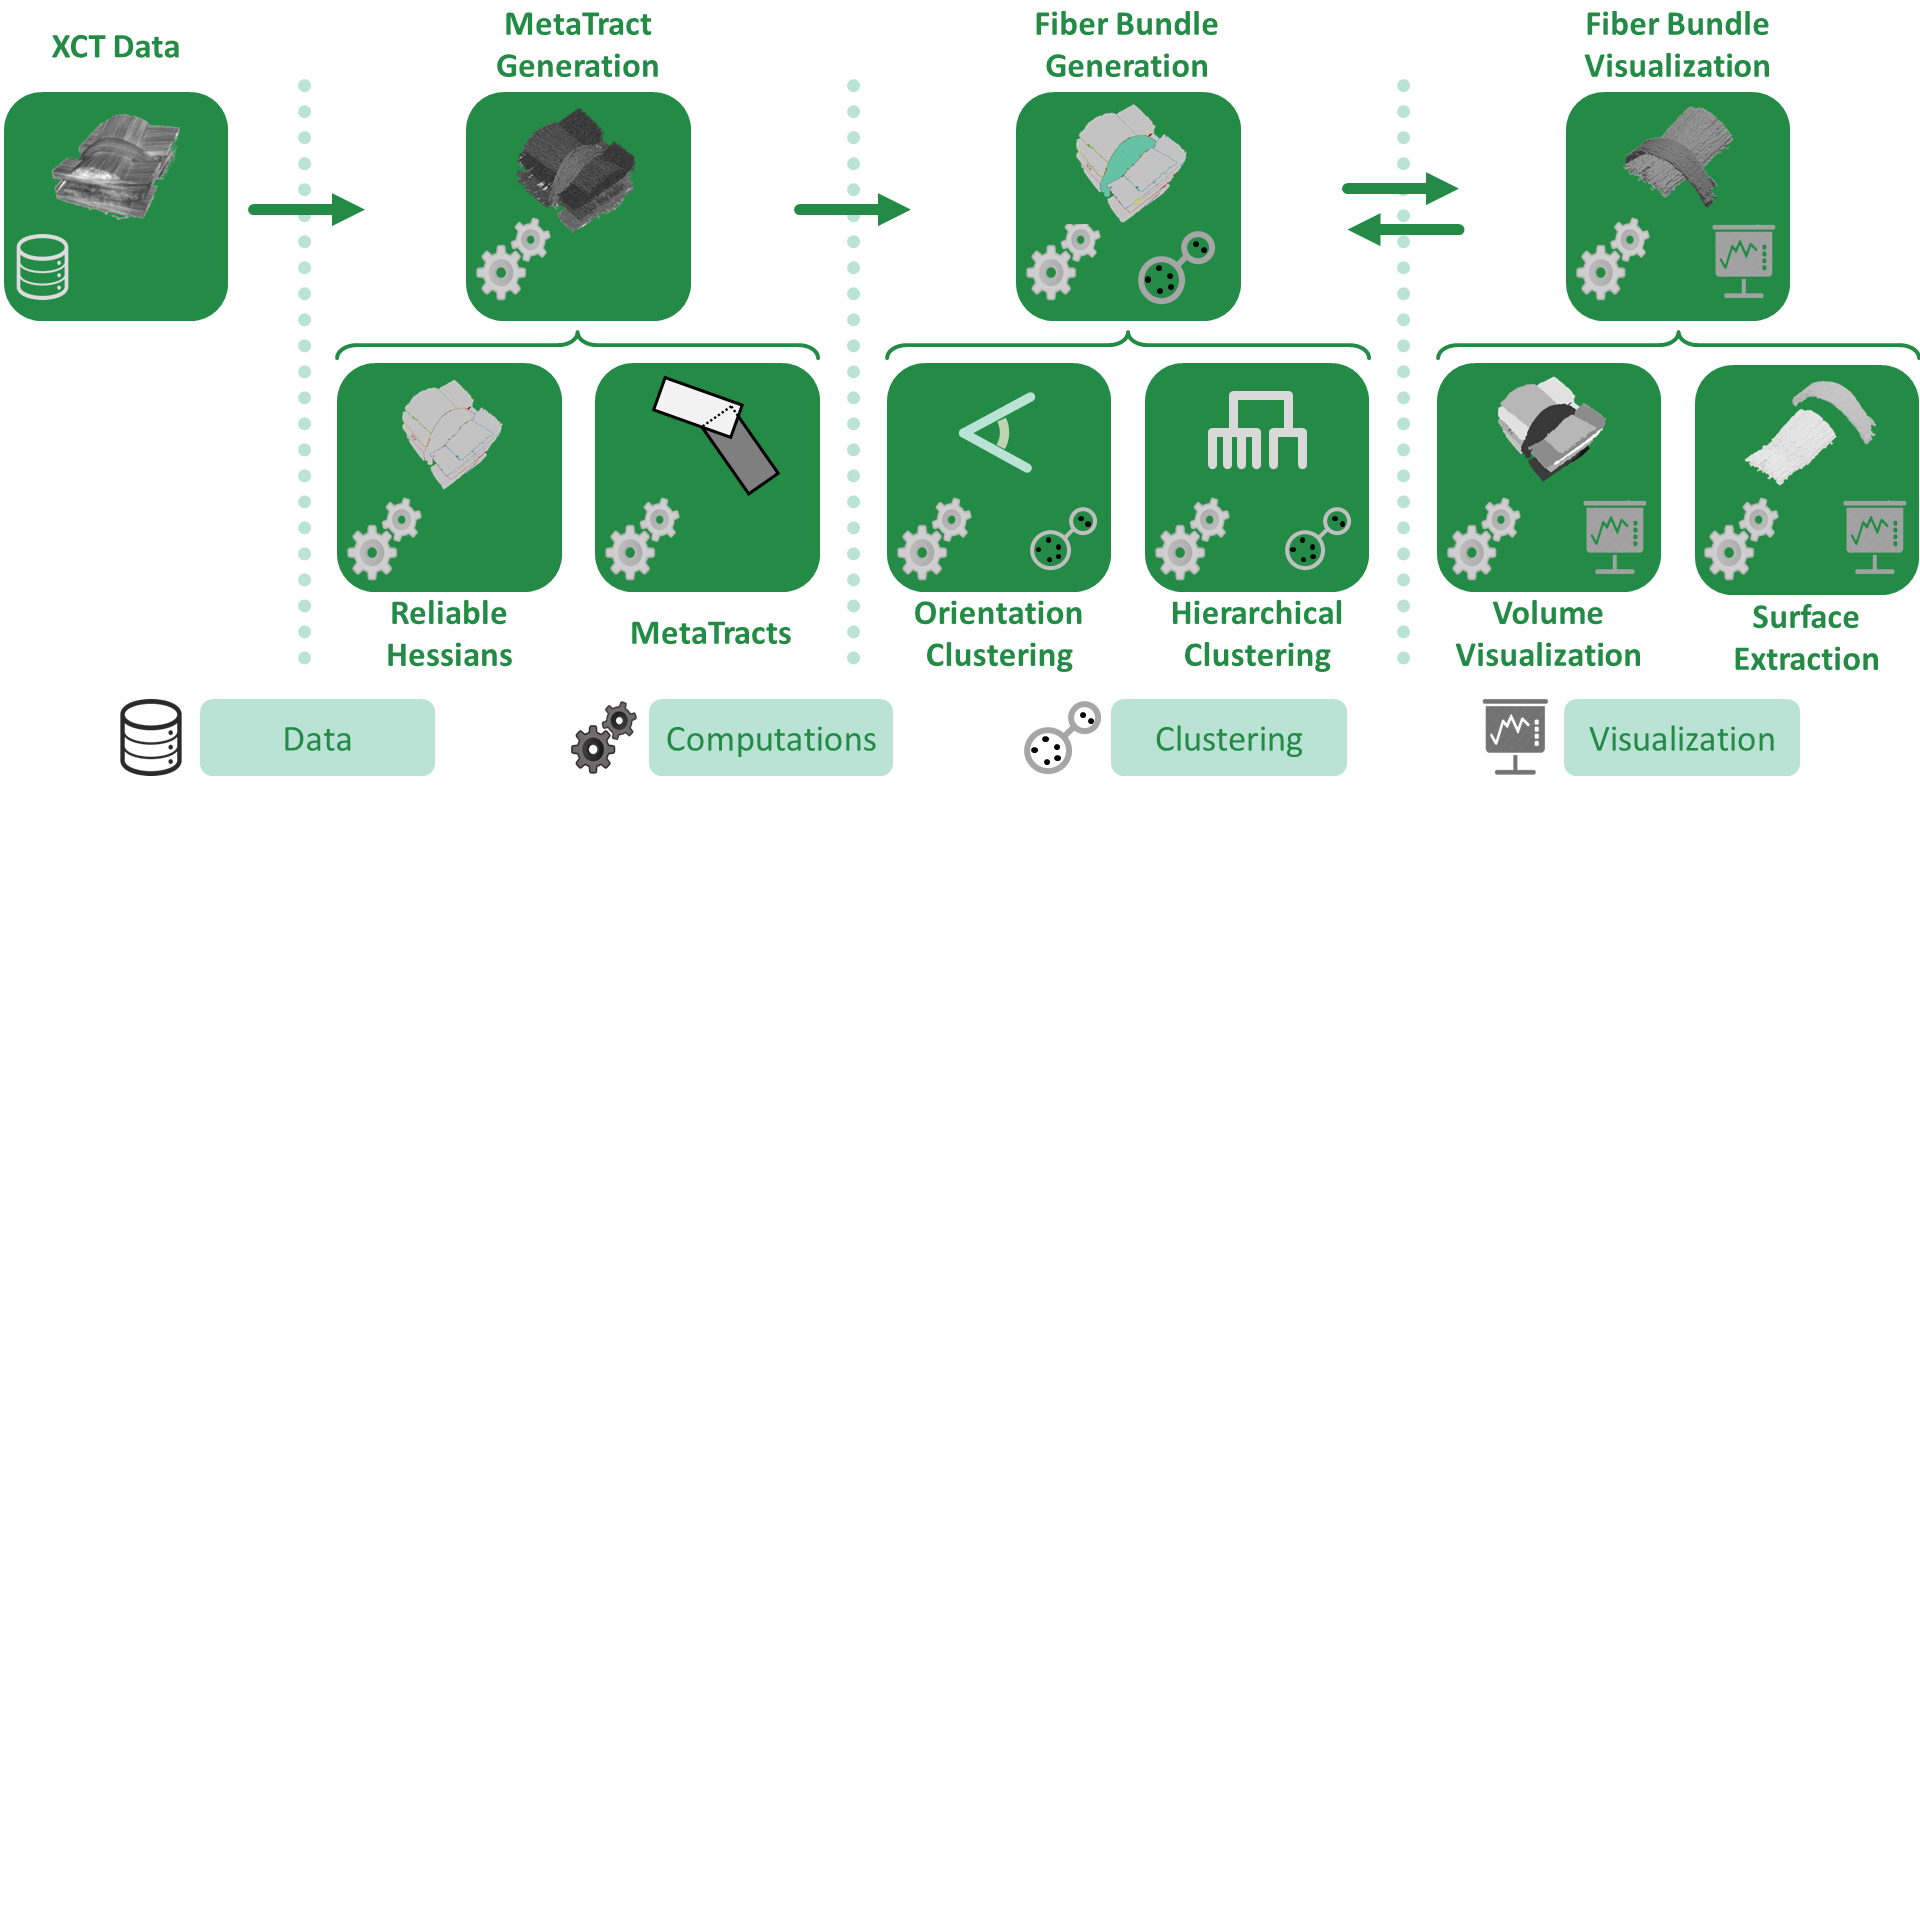
\includegraphics[width=0.5\textwidth,  trim = 0mm 300mm 0mm 0mm, clip,]{imagesMT2014/image_algo}
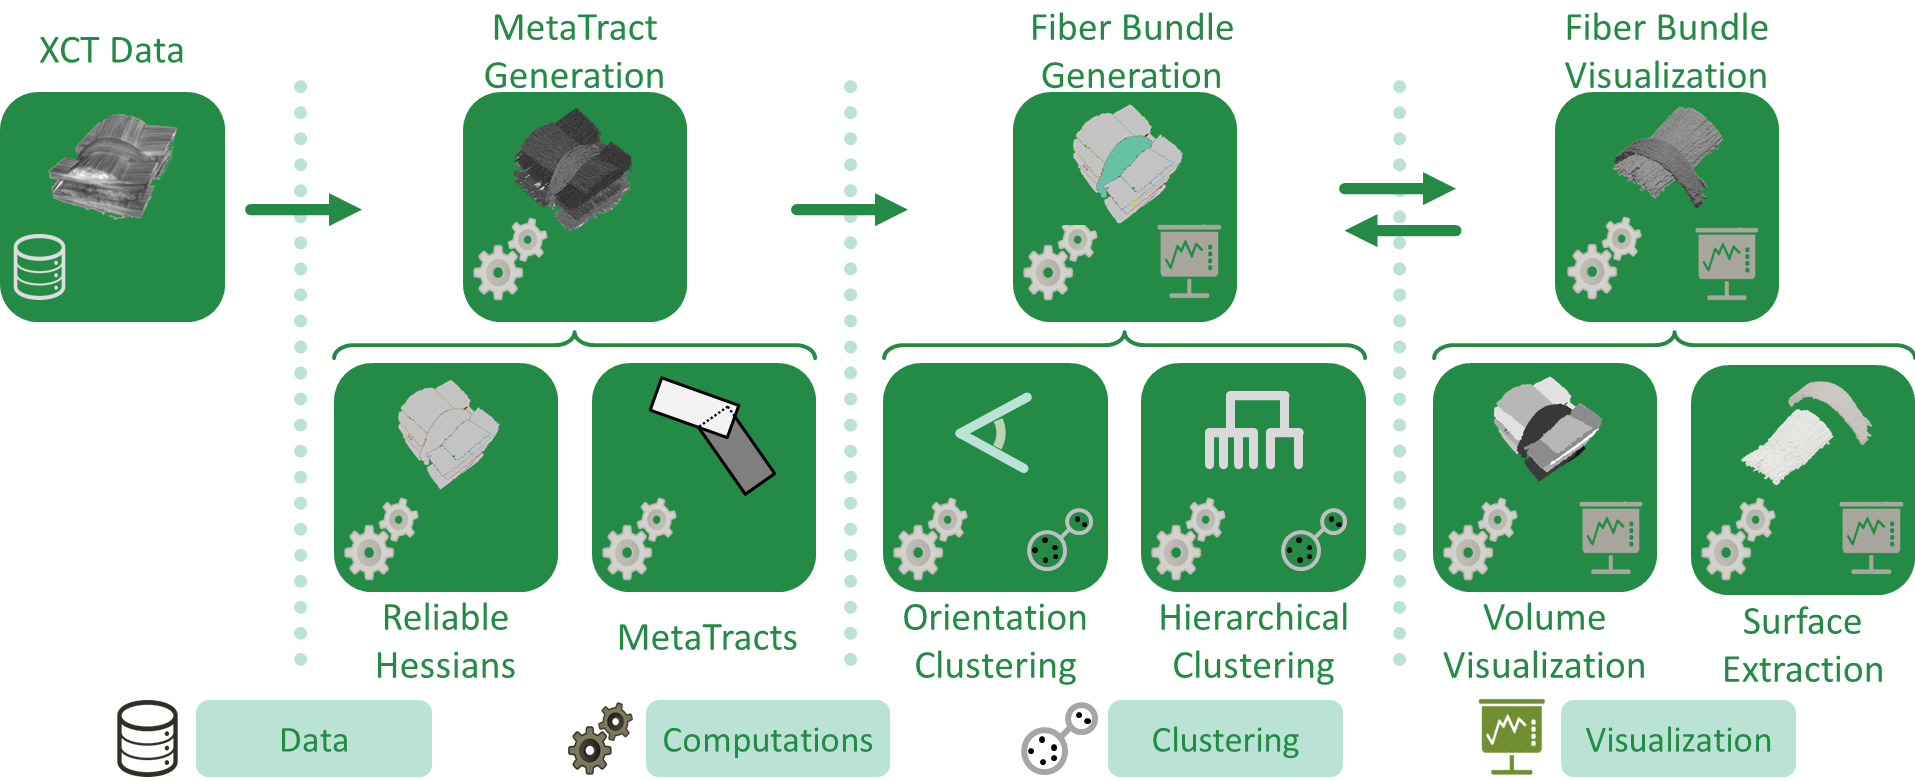
\includegraphics[width=0.5\textwidth]{images_pvis/workflow.png}
\caption{Flow chart of the MetaTracts approach for fiber bundle extraction}
\label{fig:flowchart}
\end{figure}

Figure \ref{fig:flowchart} shows our pipeline. The approach consists of multiple steps. MetaTracts generations  is explained in Section.~\ref{sec:approach} and  finding plausible fiber bundles in Section~\ref{subsec:fiber-bundles}, Section~\ref{sec:vis} talks about visualization extensions.
%\subsection {Extracting MetaTracts}
%\label{subsec:ExFiberCyl}
%We explain the different steps of MetaTracts extraction.


\subsection {Reliable Hessians}
\label{subsec:rh}

The input to the first stage of our pipelines, is the original scalar dataset in a uniform lattice grid in $\mathbb{R}^3$. As output, each grid location becomes associated with a vector representing the local orientation and a real value [0,1] which represents a measure of the reliability of the local orientation. We approximate the local orientation by eigenvalue analysis of the Hessian matrix computed at each voxel. The principal directions, in which the local second order structure of the image can be decomposed, are given by the eigen decomposition of the Hessian matrix which describes the local curvature.
The eigenvector corresponding to the smallest eigenvalue gives the direction along which the curvature is smallest. This direction coincides with the direction of the tubular structure.

Frangi et al.~\cite{Frangi1998} introduced a process that searches for geometric structures which are tubular. They define a measure based on two geometric ratios of the second order ellipsoid given by the local Hessian matrix to measure the ``vesselness'' criterion.  In order to determine reliable Hessians, we compute a similar metric. We include their work here for completeness and direct the reader to ~\cite{Frangi1998} for details. Let $\lambda_{K}$ be the eigenvalue with the $K^{th}$ smallest magnitude. Here $|{\lambda}_{1}| \leq| {\lambda}_{2}|\leq| {\lambda}_{3}| $ are the eigen values of the Hessian matrix. Specifically, a pixel belonging to a vessel region will have small $\lambda_{1}$ ($|\lambda_{1}|\approx 0$) and $\lambda_{2}$, $\lambda_{3}$ of large magnitude and of equal sign($|\lambda_{1}| \ll |\lambda_{2}|$ and $|\lambda_{2}|\approx |\lambda_{3}|$). The sign indicates if the vessel is bright in a dark background or dark in a bright background. In our case the individual fibers are bright ($\lambda_2,\lambda_3 < 0$).  The following measures are defined in their work~\cite{Frangi1998}.  
\begin{equation}\label{RA}
\mathcal{R_{A}}=\frac{\textrm{Largest  Cross Section}\big/ \pi}{{\textrm{Largest Axis Semi-length}}^{2}}=\frac{|\lambda_{2}|}{|\lambda_{3}|}
\end{equation}
\begin{equation}\label{RB}
\mathcal{R_{B}}=\frac{\textrm{Volume}\big/ (4\pi \big/ 3)}{{(\textrm{Largest Cross Section Area}\big/ \pi)}^{\frac{3}{2}}}=\frac{|\lambda_{1}|}{\sqrt{|\lambda_{2}\lambda_{3}|}}
\end{equation}
In equation~\ref{RB}, $\mathcal{R_{B}}$ provides a measure of deviation from a blob like structure while in equation~\ref{RA}, $\mathcal{R_{A}}$ distinguishes between plate-like and line-like structure. Grey-scale variations and close proximity of the fibers in our data make the Hessians computed at each voxels susceptible to errors. Thus we compute a measure, ``equal" to the ``vesselness'' measure to determine which locations in the volume provide reliable local orientation.
$$
R_{H} = \left\{ \begin{array}{ccc}
 0 & \mbox{ if $\lambda_{2}>0$ or $\lambda_{3}>0$} \\
  (1-e^{\frac{\mathcal{-R_{A}}^{2}}{2\alpha^{2}}})
  (e^{\frac{\mathcal{-R_{B}}^{2}}{2\beta^{2}}}) (1-e^{\frac{-s^2}{2c^2}}) &\mbox{ otherwise}
       \end{array} \right.
$$
Variable $s$ is the Frobenius norm of the Hessian matrix. The value  of $(1-e^{\frac{-s^2}{2c^2}})$ will be low in regions with no structure. The utility of the vesselness is a little different in our framework than Frangi et al.~\cite{Frangi1998}.
First, in biology vesselness is computed for different scales because the vessels can be of different sizes. In our case, usually the width of individual fibers are known a priori.
Second, and more importantly, we do not have clear tubular structures embedded in a dark contrast matrix such as in blood vessels.
Instead, we are trying to associate each grid location  with a probable orientation based on its local second order structure. The $R_{H}$ is interpreted as a reliability measure of the local orientation.
Grid locations where the $R_{H}$ is above a certain threshold are marked as regions with reliable orientations.
We use 0.3 as the cutoff for all our test cases. (See Section~\ref{sec:param_choices} on the choice of 0.3).
%\begin{figure}[h]
%	\centering
% \subfloat[]{ \includegraphics[width=0.2\textwidth,clip=true,trim=0cm 1cm 0cm 1cm]{imagesMetaTracts/crop-13-tracks-hess.eps}\label{fig:r_h:a}}
%   \subfloat[]{\includegraphics[width=0.25\textwidth,scale=0.2]{imagesMetaTracts/rh-1c-anno.png}\label{fig:r_h:b}}
%  \caption{Reliable Hessians: (a) Shows $R_{H}$ colored according to the absolute value of the normalized major eigenvector (local orientation) mapped to RGB color space. Fig~\ref{fig:r_h:b} shows part of a single slice where two bundles along Z(blue)axis and X(red)axis meet. Spurious specks shows that the local orientation is still noisy. Black denotes area below the $R_H$ threshold.}\label{fig:r_h}
%\end{figure}
%\begin{figure}
%\centering
%\includegraphics[width=0.4\textwidth,scale=0.1,clip=true,trim=0cm 1cm 0cm 1cm]{imagesMetaTracts/crop-13-hess-2}
% \caption{Reliable Hessians: Left, shows $R_{H}$ colored according to the absolute value of the normalized major eigenvector (local orientation) mapped to RGB color space. Right, shows a single slice along the X axis. Spurious specks shows that the local orientation is still noisy. Black denotes area below the $R_H$ threshold.}\label{fig:r_h}
%\end{figure}
In Figure~\ref{fig:reliable_hessian} we see the intermediate results of the local orientation computation only at locations where $R_{H}$ is greater than the cutoff threshold. The unit vector representing the principal direction has been mapped to RGB color space. Figure~\ref{fig:reliable_hessian}A shows the entire data set. Regions where the principal direction is parallel to the X axis are red in color, directions parallel to Y are green and those parallel to the Z are blue. Figure~\ref{fig:reliable_hessian}B and C show 2D slices along the Z and X axis respectively. Figure~\ref{fig:reliable_hessian}D shows a close up (region similar to Figure~\ref{fig:data-char}D). Note, the dark regions within a bundles are regions where the $R_H$ is less than the threshold. The bundles are not uniformly colored, the Hessians and the corresponding directions are noisy.

% We note some intrinsic differences between the DTI and our XCT data. The Hessian computation works best when the tubular structures are well separated from the surrounding, unfortunately, this is not the case for our data (Fig.~\ref{fig:r_h}). Thus the local orientation at each voxel for XCT data is inherently more noisy (Fig.~\ref{fig:r_h} Right) than those computed from eigen analysis of diffusion tensors in DTI datasets.
 
We note some intrinsic differences between the DTI and our XCT data. Fiber traces can be created in DTI using a standard fiber tracking algorithm following the principal direction of diffusion using a fourth order Runge-Kutta method~\cite{Brun2003}. The principal direction based on the Hessian matrix works best when the tubular structures are well separated from the surrounding, this is not the case for our data. The local orientaion at each voxel is inherently more noisy. Thus techniques popular in DTI cannot be directly applied in XCT data.

%
\begin{figure}[tb]
\centering
%\includegraphics[width=0.45\textwidth]{images_pvis/figure3}
\includegraphics[width=0.5\textwidth,  trim = 0mm 90mm 0mm 0mm, clip]{images_pvis/figure3}
\caption{Reliable Hessians. (A) Colored according to Orientation vector mapped to RGB. (B) 2D slice along Z and (C) along X axis. (D) close up of the region marked in green in C.}
\label{fig:reliable_hessian}
\end{figure}


\subsection {MetaTracts properties and description} 
\label{subsec:mtprop}
%\begin{figure*}
%  \centering
%  \subfloat[Meta tract generation in 2D]{\includegraphics[width=0.5\linewidth]{imagesMetaTracts/algo-1b.eps}}
%  \subfloat[Orientation based similarity measure]{\includegraphics[width=0.5\linewidth]{imagesMetaTracts/algo-1c.eps}}
%  \caption{Simplified examples of meta tract generation process and orientation based similarity measure}
%  \label{fig:algo}
%\end{figure*}
%\begin{figure*}
%  \centering
%  \subfloat[]{\includegraphics[width=0.2\textwidth]{imagesMetaTracts/algo-1d}}
%  %\subfloat[Orientation based similarity measure]{\includegraphics[width=0.5\linewidth]{imagesMetaTracts/algo-1c.eps}}
%  \caption{Simplified example of meta tract generation process.}
%  \label{fig:algo}
%\end{figure*}
The input to this step is a grid in $\mathbb{R}^3$ where each grid point is associated with a normalized local orientation and a corresponding $R_H$ value.
Traditional integral curve based techniques cannot be used to extract fiber bundle traces from the reliable Hessians because of the spurious nature of the Hessian based local orientation. Thus instead of building fiber traces, we wish to find an abstract representation of the fibers. We build on the key assumptions on the data, namely `local orientation' and `connectivity' while taking into account the noise and lack of resolution. We do this by interpreting the underlying geometric structure of the fibers as a set of polylines (cylinders). MetaTacts  are a coarse and simple approximation of integral curves in the form of a continuous chain of cylindrical tubes in $\mathbb{R}^3$ traversing the fiber bundles embedded in the input data. MetaTracts share the following \textit{properties}:

\begin{enumerate}
\item{Each MetaTract is associated with a continuous set of cylinders.}
\item{Each MetaTract is associated with a start point which is a grid vertex.}
\item{Each individual cylinder in a MetaTract has a constant length, a constant radius and a start point (which is also a grid vertex).}
\item{Each cylinder in a MetaTract (except for the first one) is connected to the previous cylinder at its start point.}
\item{Each cylinder is locally parallel to the local orientation at it's start point.}
\end{enumerate}


% $N_{p}$ (Fig.~\ref{fig:algo} provides an overview). Let $C_{p}$ be the grid point associated with the current cylinder. We insert a subset of the grid points $G_{q}$ that lie within the cylinder into a priority queue. The priority is defined by equation \ref{eqn:algo_1}. In Equation \ref{eqn:algo_1}, $angle$ refers to the angle between the local orientation at the current point $C_{p}$ and the grid point $G_{q}$. $PerpDist$ refers to the perpendicular distance between the $G_{q}$ and $C_{p}$ projected along the direction of the local orientation $N_{p}$. We only insert a grid point $G_{q}$ in the priority queue if the $angle$ is less than 20 degrees and the $PerpDist$ is at least 0.5. This ensures that points with obvious spurious local orientation or points which are very close to  $C_{p}$ are not put in to the queue. This simple check ensures our memory requirements are not excessive.


\subsection {MetaTracts generation}
\label{subsec:MetaTracts-generation}
In $\mathbb{R}^2$ all the above properties hold except that cylinders are replaced by rectangles. We explain the process of MetaTracts generation in $\mathbb{R}^2$. The procedure trivially extends to $\mathbb{R}^3$. The reliable Hessian step  generates a local orientation in $\mathbb{R}^2$ and a $R_H$[0,1]. In Figure \ref{fig:algo} all regions which have reliable Hessian less than the threshold have been marked in blue(Fig.~\ref{fig:algo}B). Let the seed point associated with the MetaTract be grid point $C_{p}$ (Property 2, Section~\ref{subsec:mtprop}). The local orientation at $C_p$ as computed in the step above is $N_P$ and is given by the dark green arrow (Fig.~\ref{fig:algo}C). We generate a rectangle of length L and radius R, the green dashed rectangle shows the rectangle generated at $C_p$ (Property 3 and 5, Section~\ref{subsec:mtprop}). 
\begin{figure}[tb]
  \begin{center}
 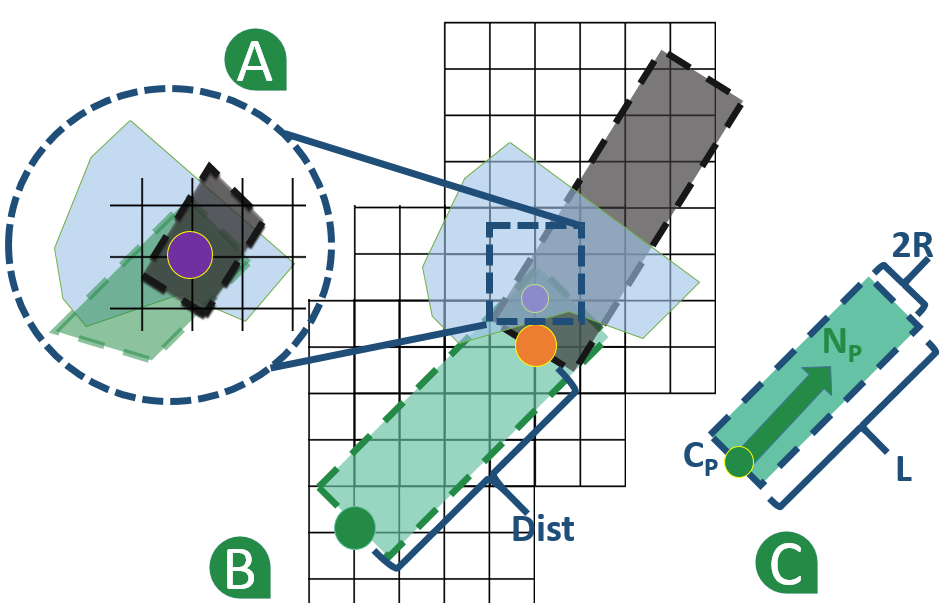
\includegraphics[ width=0.4\textwidth]{imagesMT2014/image4}
  \end{center}
  \vspace{-1em}
 \caption{MetaTracts generation: (B) MetaTract generation, region with $R_H$ less than threshold. (A) close up of marked region in (B). (C) Parts of a single MetaTract.}
  \label{fig:algo}
    \vspace{-1.5em}
\end{figure}
The set of vertices which are in the green region but not overlapped by blue are possible candidates for the start point of the next cylinder in a particular MetaTract. We call these vertices \textit{``candidate vertices"}. From these we select another grid vertex which will be the start point for the next cylinder.
%\begin{figure}
%\centering
% \includegraphics[width=0.25\textwidth]{imagesMetaTracts/angle-diff.png}
%\caption{Angle between the local orientation of two cylinders that are part of the same MetaTract.}
%\label{fig:angle-diff}
%\end{figure}
The order of the candidate vertices is based on the following characteristics:

\begin{itemize}
\item \textit{Orientation Similarity}: We want the orientation of the start points for the consecutive cylinders to have a similar orientations ($N_p$). 
\item \textit{Large distance}: We want the MetaTracts to traverse the data using as few cylinders as possible. Thus, we want the distance between $C_p$ and the start point for the next cylinder to be as large as possible. We measure distance of a candidate vertex from $C_p$ by projecting the Euclidean distance between them onto $N_p$. For example the Euclidean distance between the blue and the orange vertices projected onto $N_P$ gives distance (Figure~\ref{fig:algo}B). We refer to this perpendicular projection distance as \textit{``projected\_dist"}. 
\end{itemize}
% \begin{equation}\label{eqn:algo_1}
% d=\frac{1}{3}e^{(\frac{-angle^{2}}{\alpha^{2}})}+\frac{2}{3}(1-e^{\frac{-{PerpDist}^{2}}{\beta^{2}}})
% \end{equation}
We further define a priority for each of the candidate vertices based on the above factors.
For each cylinder in a MetaTract, we put the \textit{candidate vertices} of it in a priority queue based on Equation \ref{eqn:algo_1}.
\begin{equation}
Priority = \gamma_1 e^{(-angle^2 / \alpha^2)} + \gamma_2e^{(-projected\_dist^2 / \beta^2)}
\label{eqn:algo_1}
\end{equation}
$\gamma_1$, $\gamma_2$ are the  weights ($\mathbb{R}_{\ge 0}$)  which decide how the priority depends on the affine combination of the two factors. For all our cases we use ($\gamma_1$ = $1 / 3 $ and $\gamma_2$ = $2 / 3$). In general we suggest $\gamma_1 +\gamma_2 = 1 $ and $\gamma_1 \leq \gamma_2$). At each iteration we pick the top element in the priority queue generate the corresponding cylinder and repeat the steps. Essentially, Equation~\ref{eqn:algo_1}, selects a grid point which is the furthest from the current point and going in a similar direction. This gives it the advantage of tackling noise/errors in local orientation better than integral curves by looking at multiple choices for vertices and avoiding intra cell interpolation in an already noisy environment. 
 
In this particular example in Figure~\ref{fig:algo}(B) we select the orange grid vertex next and repeat the process. We do not select the purple vertex (Figure~\ref{fig:algo}(C)) because it is not a candidate vertex. If we generate tracts that have erroneous local orientations they will not be able to find further possible candidate vertices and will be of short length. Short tracts are then removed. The MetaTracts generated are shown in Figure~\ref{fig:length_distribution}A. The MetaTracts are colored with the mean orientation direction mapped to the RGB space. That consistent orientation is a key intrinsic feature in the data becomes visually pronounced.
We apply uniform, dense seeding to the XCT volume data to trace and generate the tracts of fiber bundles. Fig.~\ref{fig:length_distribution}(B) shows the MetaTracts of a particular bundle colored according to their length.
MetaTracts in a given fiber bundle do not extend the full length of the bundle. MetaTracts may have different lengths and may partially overlap.
 
% \begin{figure}[h]
% \centering
% 	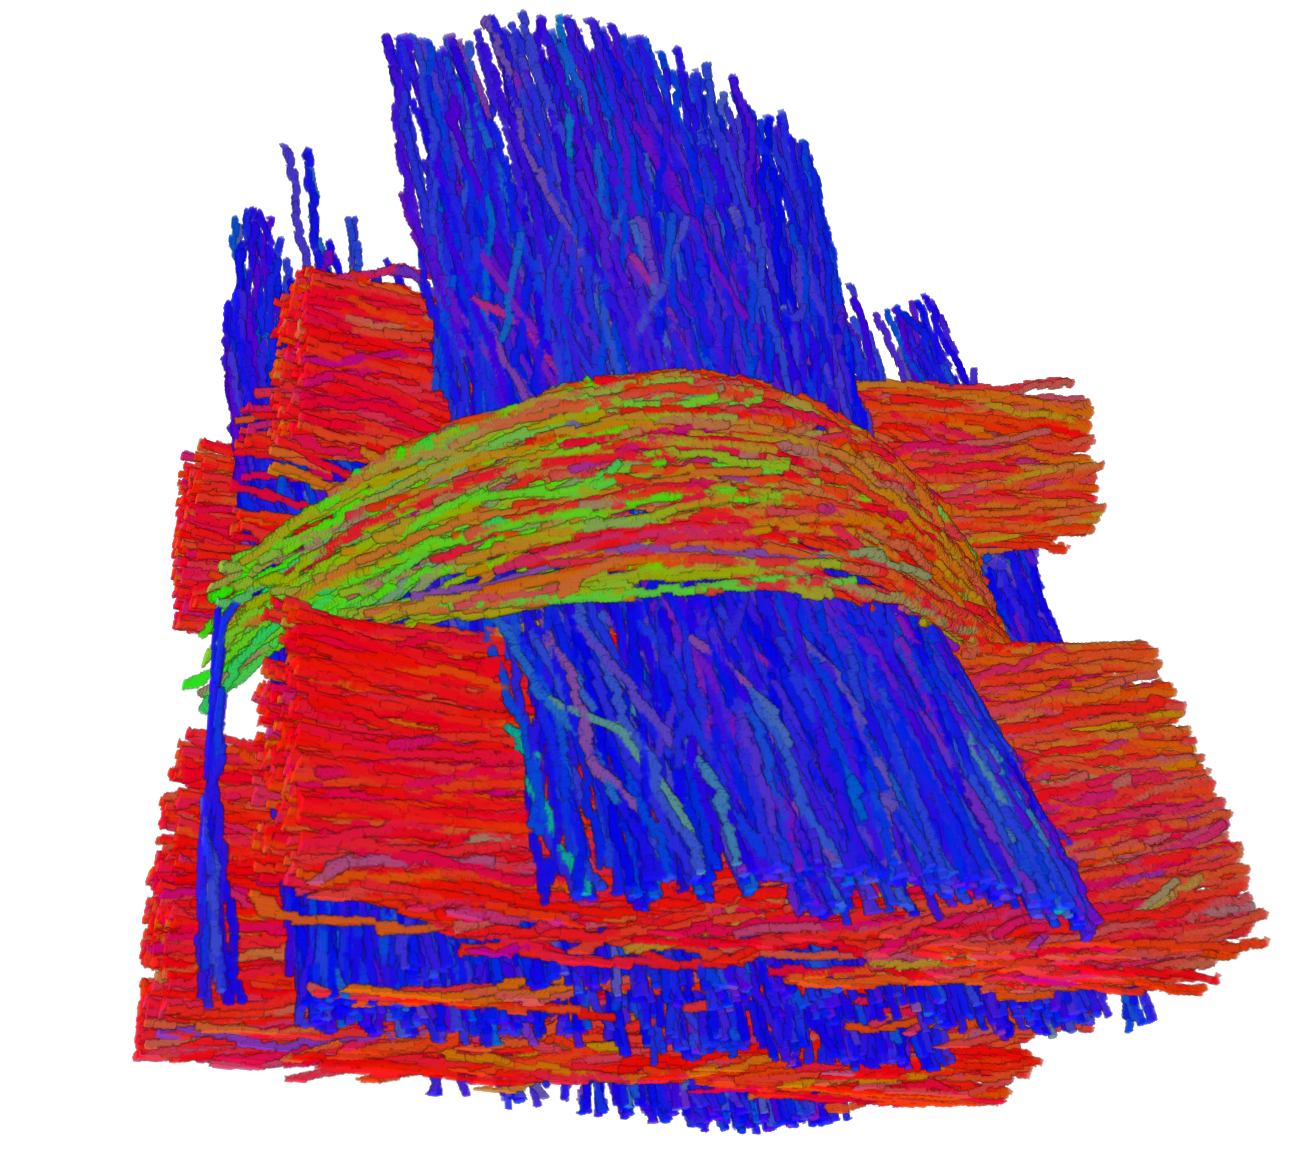
\includegraphics[ trim = 2cm 2cm 2cm 2cm, clip=true, width=0.3\textwidth]{imagesMT2014/MT_crop16_MT.png}
% 	\caption{MetaTracts, colored according to mean orientation mapped to RGB space}
% \label{fig:meta-tract}
% \end{figure}
 
%\begin{figure}
%  \centering
%  {\includegraphics[width=0.2\textwidth]{imagesMetaTracts/crop-13-tracks-1.eps}}
%  \caption{MetaTracts generated from one of our data sets. Each MetaTracts consists of cylinders. The mean local orientation, computed as the mean of the local orientations at the start point of each cylinder composing a particular MetaTract is mapped to the RGB space }\label{fig:meta-tracts}
%\end{figure}
%
 
%\begin{figure*}[htp]
%  \centering
%  \subfloat[]{\includegraphics[width=0.25\linewidth]{imagesMetaTracts/rplot-crop13.eps}}
% % \subfloat[]{\includegraphics[width=0.28\linewidth]{imagesMetaTracts/crop-13-tracks-clus-b.eps}}
%    \subfloat[]{\includegraphics[width=0.22\linewidth]{imagesMetaTracts/crop-13-tracks-clus-b-anno.png}}
%  \subfloat[]{\includegraphics[width=0.25\linewidth]{imagesMetaTracts/crop-13-tracks-clus-a.eps}}
%  \caption{Results from orientation based and hierarchical clustering. (a) shows the result of the K-means clustering with the data points projected to the top three Eigenvectors as the major axes, (b) shows the MetaTracts colored according to clustering results in (a), the corresponding clusters divide the MetaTracts according to their major orientation. (c) shows the result of hierarchical clustering of the results in (b), each orientation cluster (in this case 2) was divided into 7 classes.}\label{fig:clustering}
%\end{figure*}

%\begin{figure}
%  \centering
%  \subfloat[]{\includegraphics[width=0.22\textwidth,clip=true,trim=1cm 0cm 1cm 2cm]{imagesMetaTracts/rplot-crop13.eps}}
% % \subfloat[]{\includegraphics[width=0.28\linewidth]{imagesMetaTracts/crop-13-tracks-clus-b.eps}}
%    \subfloat[]{\includegraphics[width=0.3\linewidth,,clip=true,trim=1cm 0cm 2cm 0cm]{imagesMetaTracts/crop-13-tracks-clus-b-anno.png}}
%  \subfloat[]{\includegraphics[width=0.4\linewidth]{imagesMetaTracts/crop-13-tracks-clus-a.eps}}
%  \caption{Results from orientation based and hierarchical clustering. (a) The result of the K-means clustering with the data points projected to the top three eigenvectors as the major axes. (b) MetaTracts colored according to clustering results in (a). Corresponding clusters dividing the MetaTracts according to their two major orientations. (c) The result of hierarchical clustering of the results in (b), The two orientation clusters are divided into seven classes.}\label{fig:clustering}
%\end{figure}

%\subsection {Seeding}

%We apply uniform, dense seeding to the XCT volume data to trace and generate the tracts of fiber bundles.
%For our result we add a constraint. Only those grid vertices which have reliable hessians (Section~\ref{subsec:rh}). This restriction limits MetaTracts to  start from regions which have some underlying geometric structure. Regions that do not have reliable Hessians have poor local orientation and will not generate long MetaTracts. We also allow the user to selectively seed particular regions more densely.

\begin{figure}[tb]
\centering
	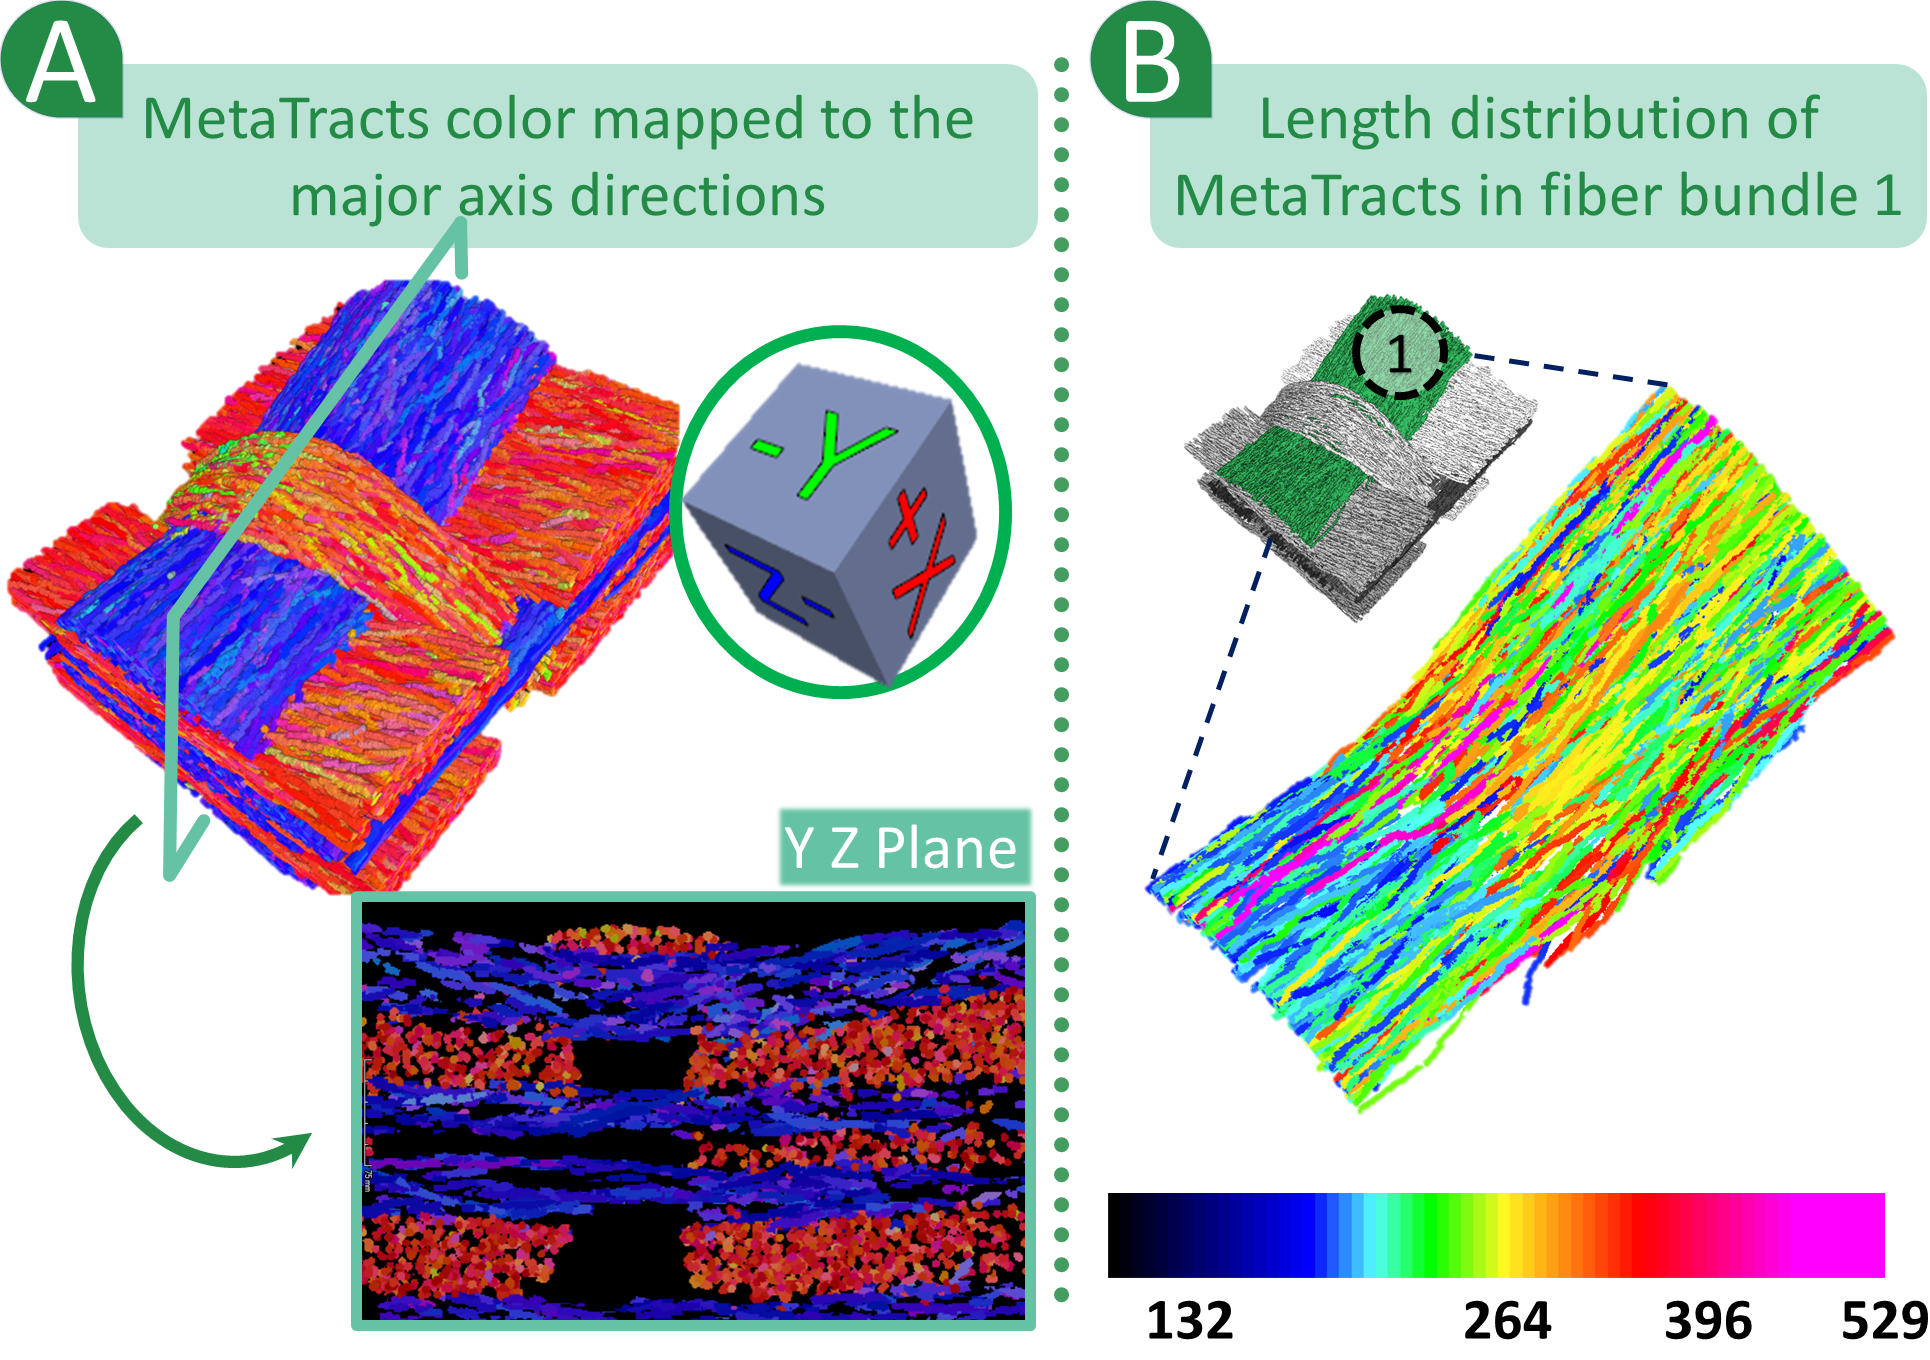
\includegraphics[width=0.45\textwidth]{images_pvis/figure5.png}
	%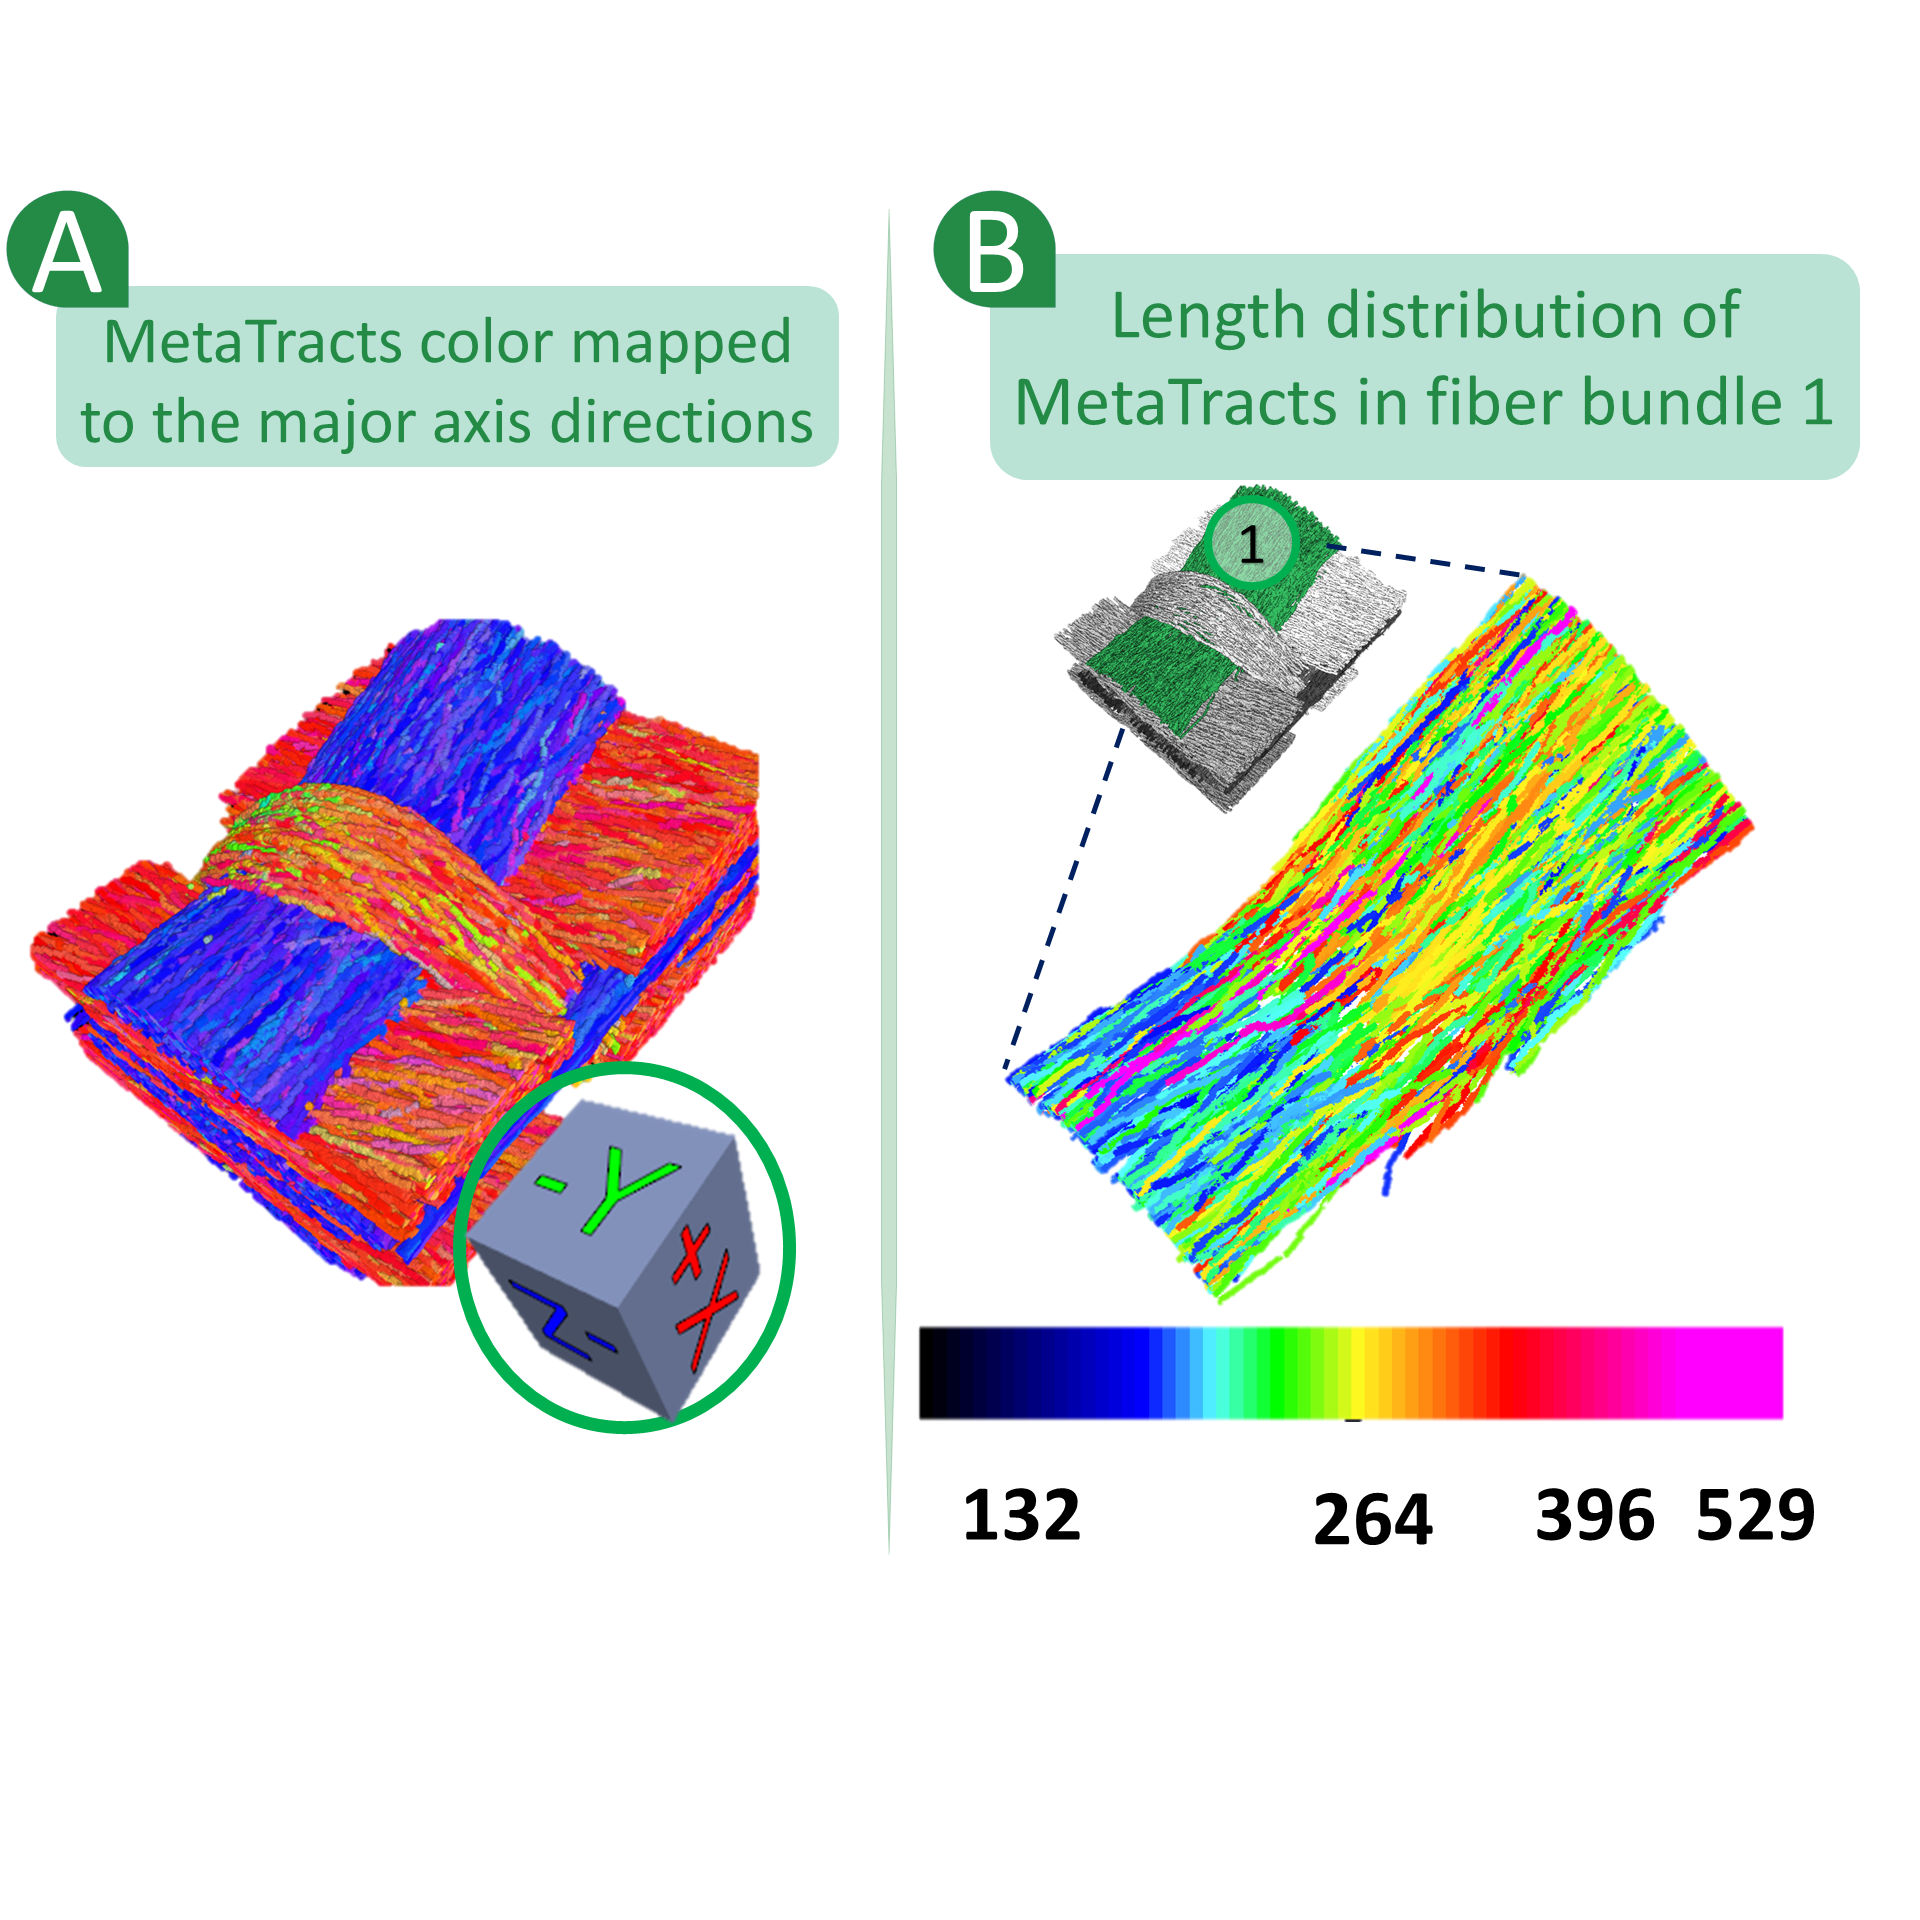
\includegraphics[width=0.45\textwidth,  trim = 0mm 100mm 0mm 50mm, clip]{imagesMT2014/image_length}
	\caption{(A) MetaTracts colored according to mean orientations. (B) length distribution of individual MetaTracts for a particular bundle.(unit for length is grid cube edge length). A single fiber bundle is made of MetaTracts of varying length}
	\label{fig:length_distribution}
\end{figure}


\section {Fiber Bundle Generation}
\label{subsec:fiber-bundles}

The output of the above step is a set of MetaTracts. The next step is to cluster the MetaTracts into bundles. 
Carbon fibers have both orientation and geometric proximity information, both of which can be used for clustering. We have found that orientation measure was very reliable while measures of geometric proximity had problems with fibers which partially overlap (Fig.~\ref{fig:length_distribution}B).  
Instead of creating a heuristic which artificially combines the orientation and geometric proximity measures, we first cluster based on orientation and then further subdivide each orientation cluster using geometric proximity.
We found that different clustering techniques performed preferably for different measures.  The two step clustering also made the problem more tractable and  the parameters intuitive for the end users. For the orientation clustering, we use dimension reduction followed by K-means clustering. We then use hierarchical clustering to further subdivide each cluster based on the geometric proximity measures. 

%However, in approaches developed for DTI fibers such as proximity based distance measures and clustering, the short comings of the fiber tracking techniques are generally not discussed and it is assumed that fibers in each bundle are of similar lengths and which traverse the data end to end. This is not the case for noisy data such as ours.
%In Figure~\ref{fig:hclust_issue_a} proximity based distance, for example mean of the minimum distances between points on MetaTracts might falsely find the red MetaTract being closer to the blue, than the orange MetaTract. 
%We also note from Figure~\ref{fig:meta-tract} and from domain knowledge that all our fibers are well separated by orientation. Thus instead of directly applying hierarchical clustering to our data,
%we first cluster based on orientation using a simple measure.
%We use domain knowledge to divide the clustering into two intuitive parts:because of the woven nature of fiber bundles in our application domain we first cluster in terms of orientation. This has the advantage of being able to separate tracts which might be close in an Euclidean space but traveling in different direction. We introduce a simple orientation based similarity measure (sec~\ref{subsec:ori-sim-mes}). Finally, for each of these clusters we re-cluster in terms of distances measured in a Euclidean space (sec~\ref{subsec:dist_clustering}).


\subsection {Orientation based clustering}
%We use the inherent features expressed as weaving pattern of our data to pre-cluster the metaTracts into the number of classes based on the major directions of the pattern.
%It is important to note that this step broadly divides the MetaTracts into classes based on the major orientations and not individual fiber bundles. 
This step divides the individual MetaTracts into classes based on their major orientations. In order to cluster MetaTracts going in same directions, we use a spectral embedding technique called Laplacian eigenmaps which was originally introduced by Belkin and Niyogi \cite{Belkin01} and later used in DTI fiber coloring~\cite{Brun2003} and fiber clustering~\cite{Brun2004}. The key notion is to find a suitable similarity measure to define the weights of an undirected weighted graph. The nodes being the data points and the edges being the weights. Then, an eigenvalue problem is solved, which maps the manifold embedded in the graph into a lower dimensional space while preserving the graph structure.
This lower dimensional space can then be clustered more efficiently than the higher dimensional space. 
Let G be the graph, we compute the eigenvalues and eigenvectors for the generalized eigenvector problem:$L\textbf{f}=\lambda D\textbf{f}$,
%\begin{equation}\label{equn:eigenMaps}
%L\textbf{f}=\lambda D\textbf{f}
%\end{equation}
where D is the diagonal weight matrix and L is the Laplacian matrix. The eigenvector \textbf{${f}_{0}$} corresponding to the eigenvalue 0 is left out and the next $m$, {\textbf{${f}_{1}$} through \textbf{${f}_{m}$}} eigenvectors are used to embed in an m-dimensional space. K-means clustering is then used to cluster in this lower dimensional space.

Brun et al.~\cite{Brun2003} based their measure on the simple assumption that two traces with similar endpoints should be considered similar. Brun et al. ~\cite{Brun2004} based their measure on a 9-D fiber descriptors. In our case, each MetaTract is a data point. We introduce a simple \textit{orientation based similarity measure}. There is no spatial information involved, just a partition of the MetaTracts based on orientation which is already inherent in the data.
Following this, given a pair of  MetaTracts, we define the edge weights between two tracts as the cosine of the maximum angle between the local orientations ($N_P$) of all pairs of start points ($C_P$) between the two MetaTracts. The edge weights give a distance matrix representing the distance between each pair of points. Using the Belkin and Niyogi algorithm we ``embed" these points in a low dimensional space where the Euclidean distance between points approximates the distance between points given by the distance matrix. 
%
%August 13 2014
%For all our tests the fibers were then embedded in a $\eta$ low dimensional space. The number of dimensions in the high dimensional space is equal to the number of datapoints or the number of MetaTracts in our case.
%For all our test cases we set $\eta$ to be five (see sec~\ref{sec:param_choices} for parameter choices for $\eta$.).
%  
We used conventional K-means for clustering this lower dimensional space. Here $K$ is supplied by domain knowledge of the number of major fiber bundle directions of the woven structure.
For our test case there are two major directions of the fiber bundles. So $K$ was set to 2. It is important to note that due to the advantages offered by the dimensionality reduction, even if there are curved fibers bundles the user has to provide just the major fiber bundle directions of the weaving pattern. Figure~\ref{fig:orientation_clustering}B shows the result of the K-means clustering with the data points projected to the top three eigenvectors as the major axes. As is expected there is a clear distinction based on fiber orientation. Figure~\ref{fig:orientation_clustering}(A,C) shows the MetaTracts colored according to clustering results.

\begin{figure}[tb] 
  \centering  	
  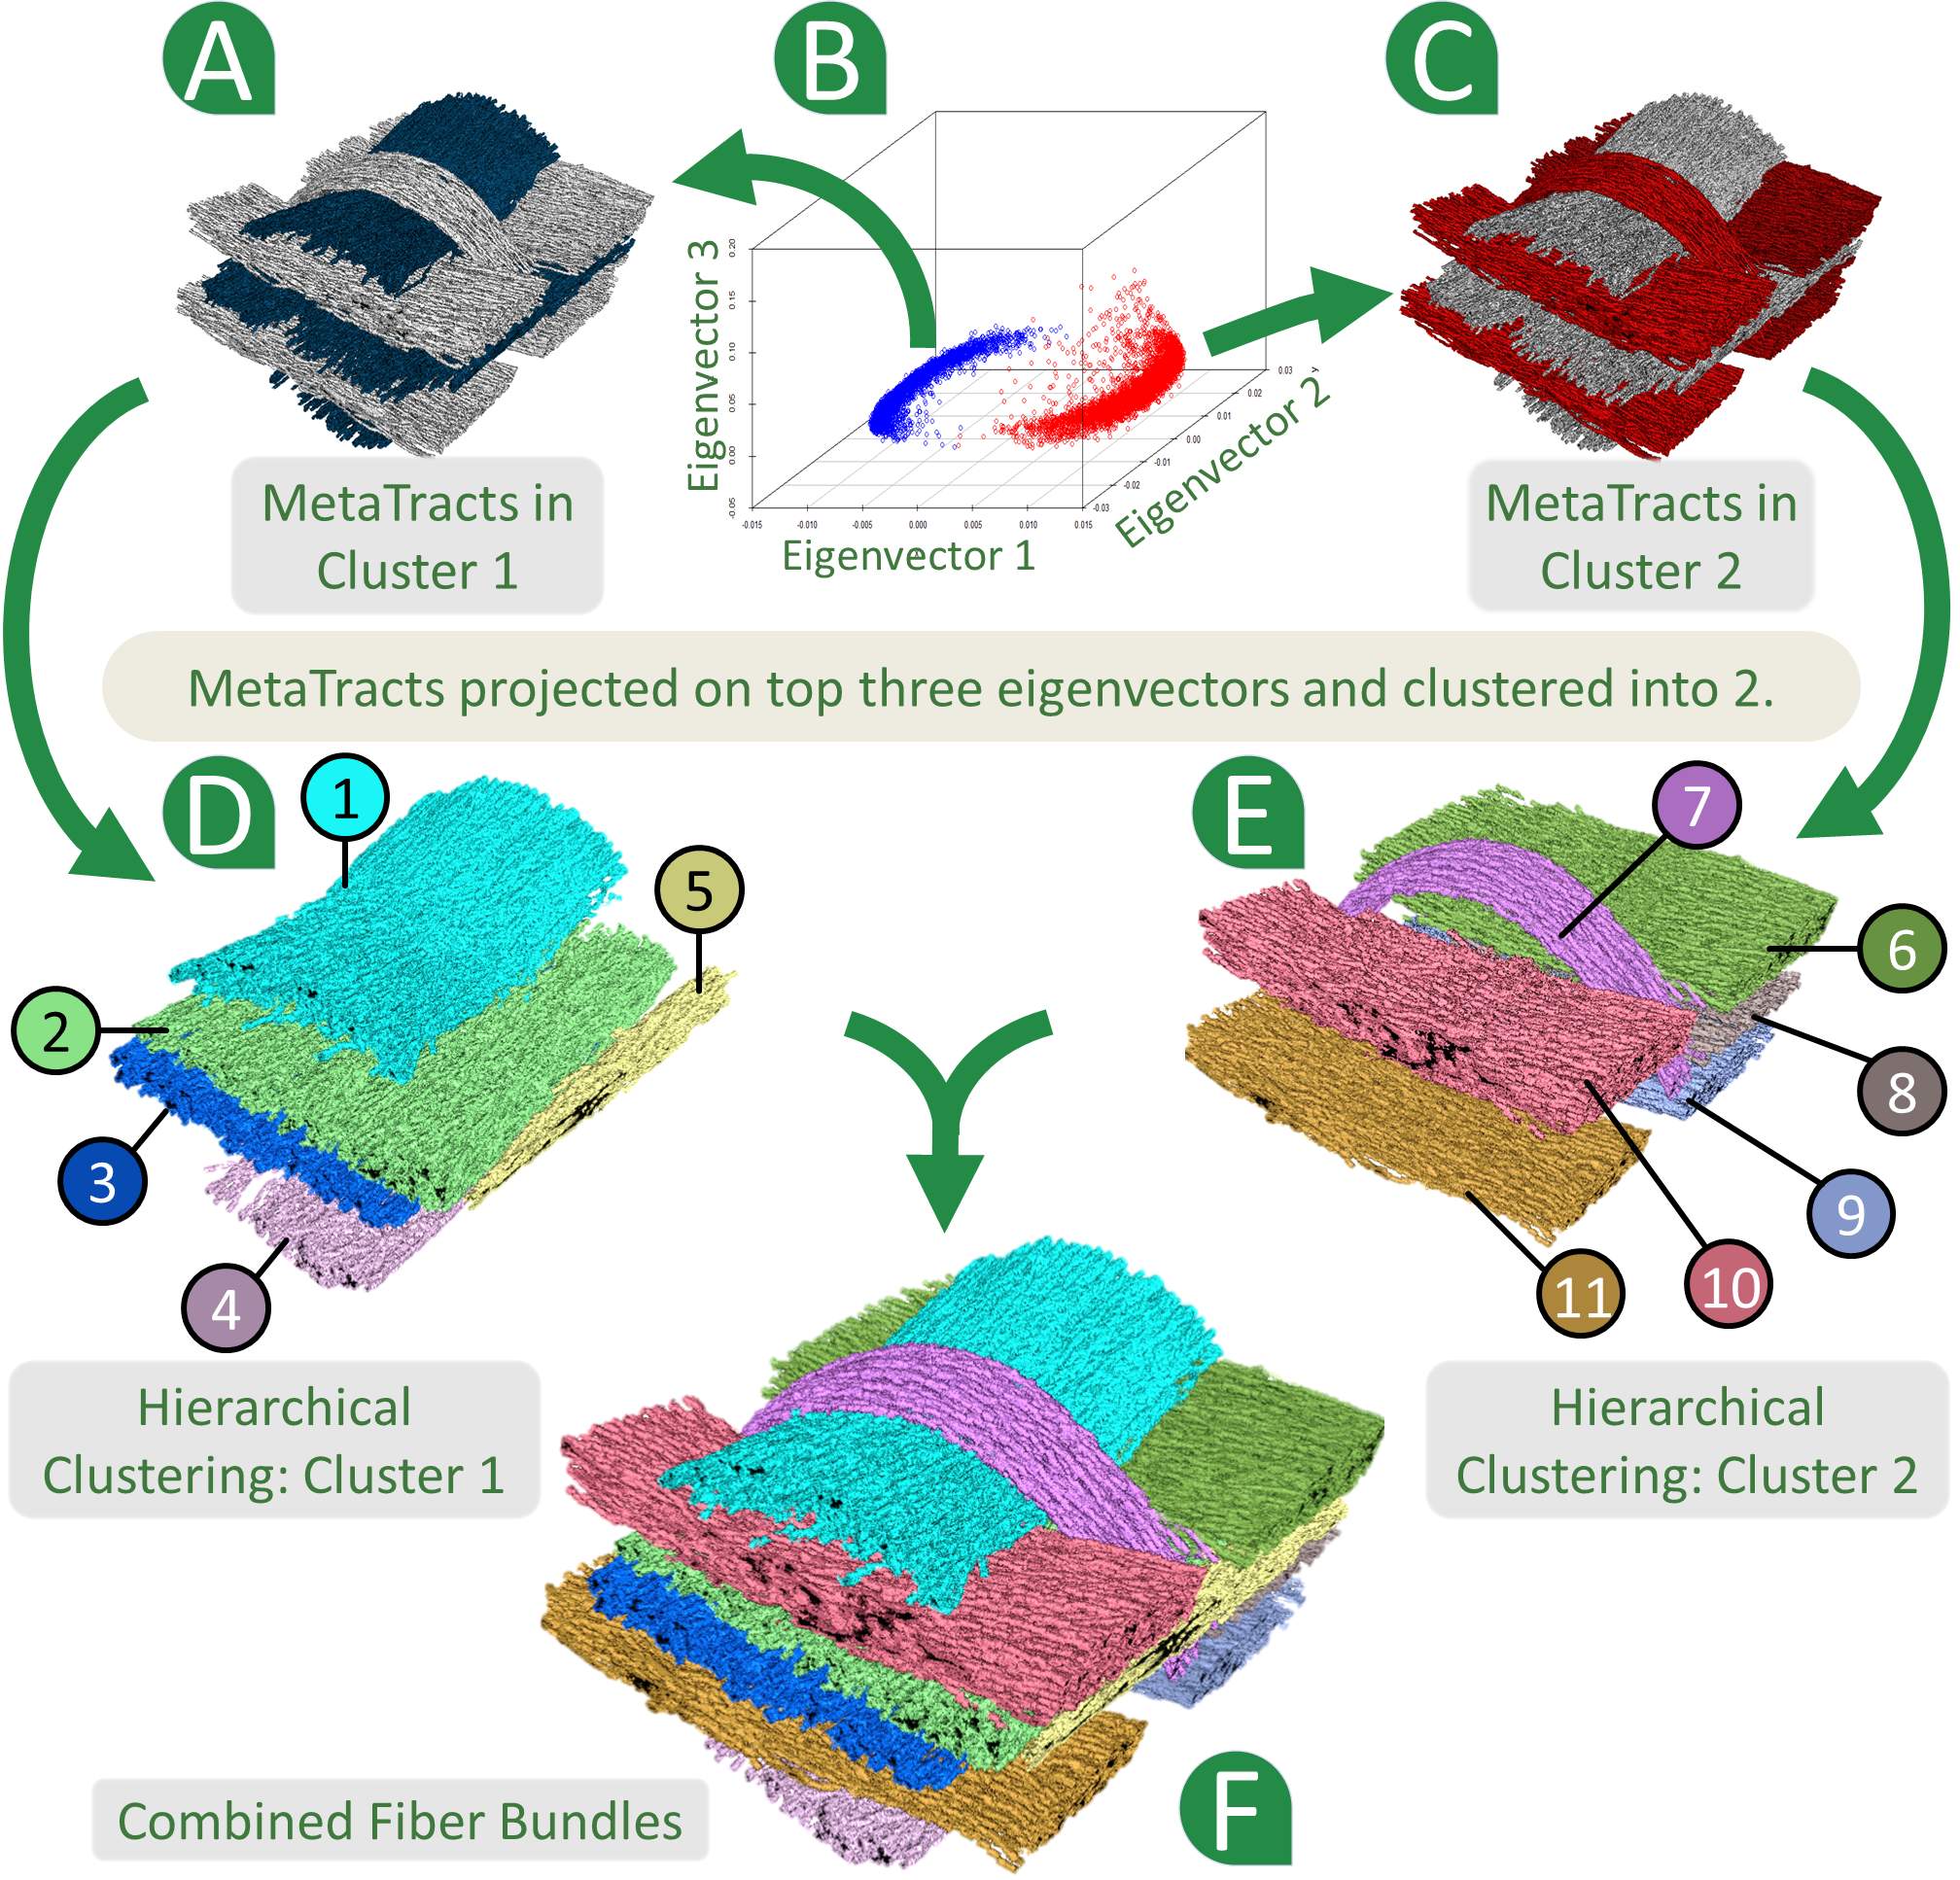
\includegraphics[width=0.5\textwidth]{images_pvis/figure6.png}
  %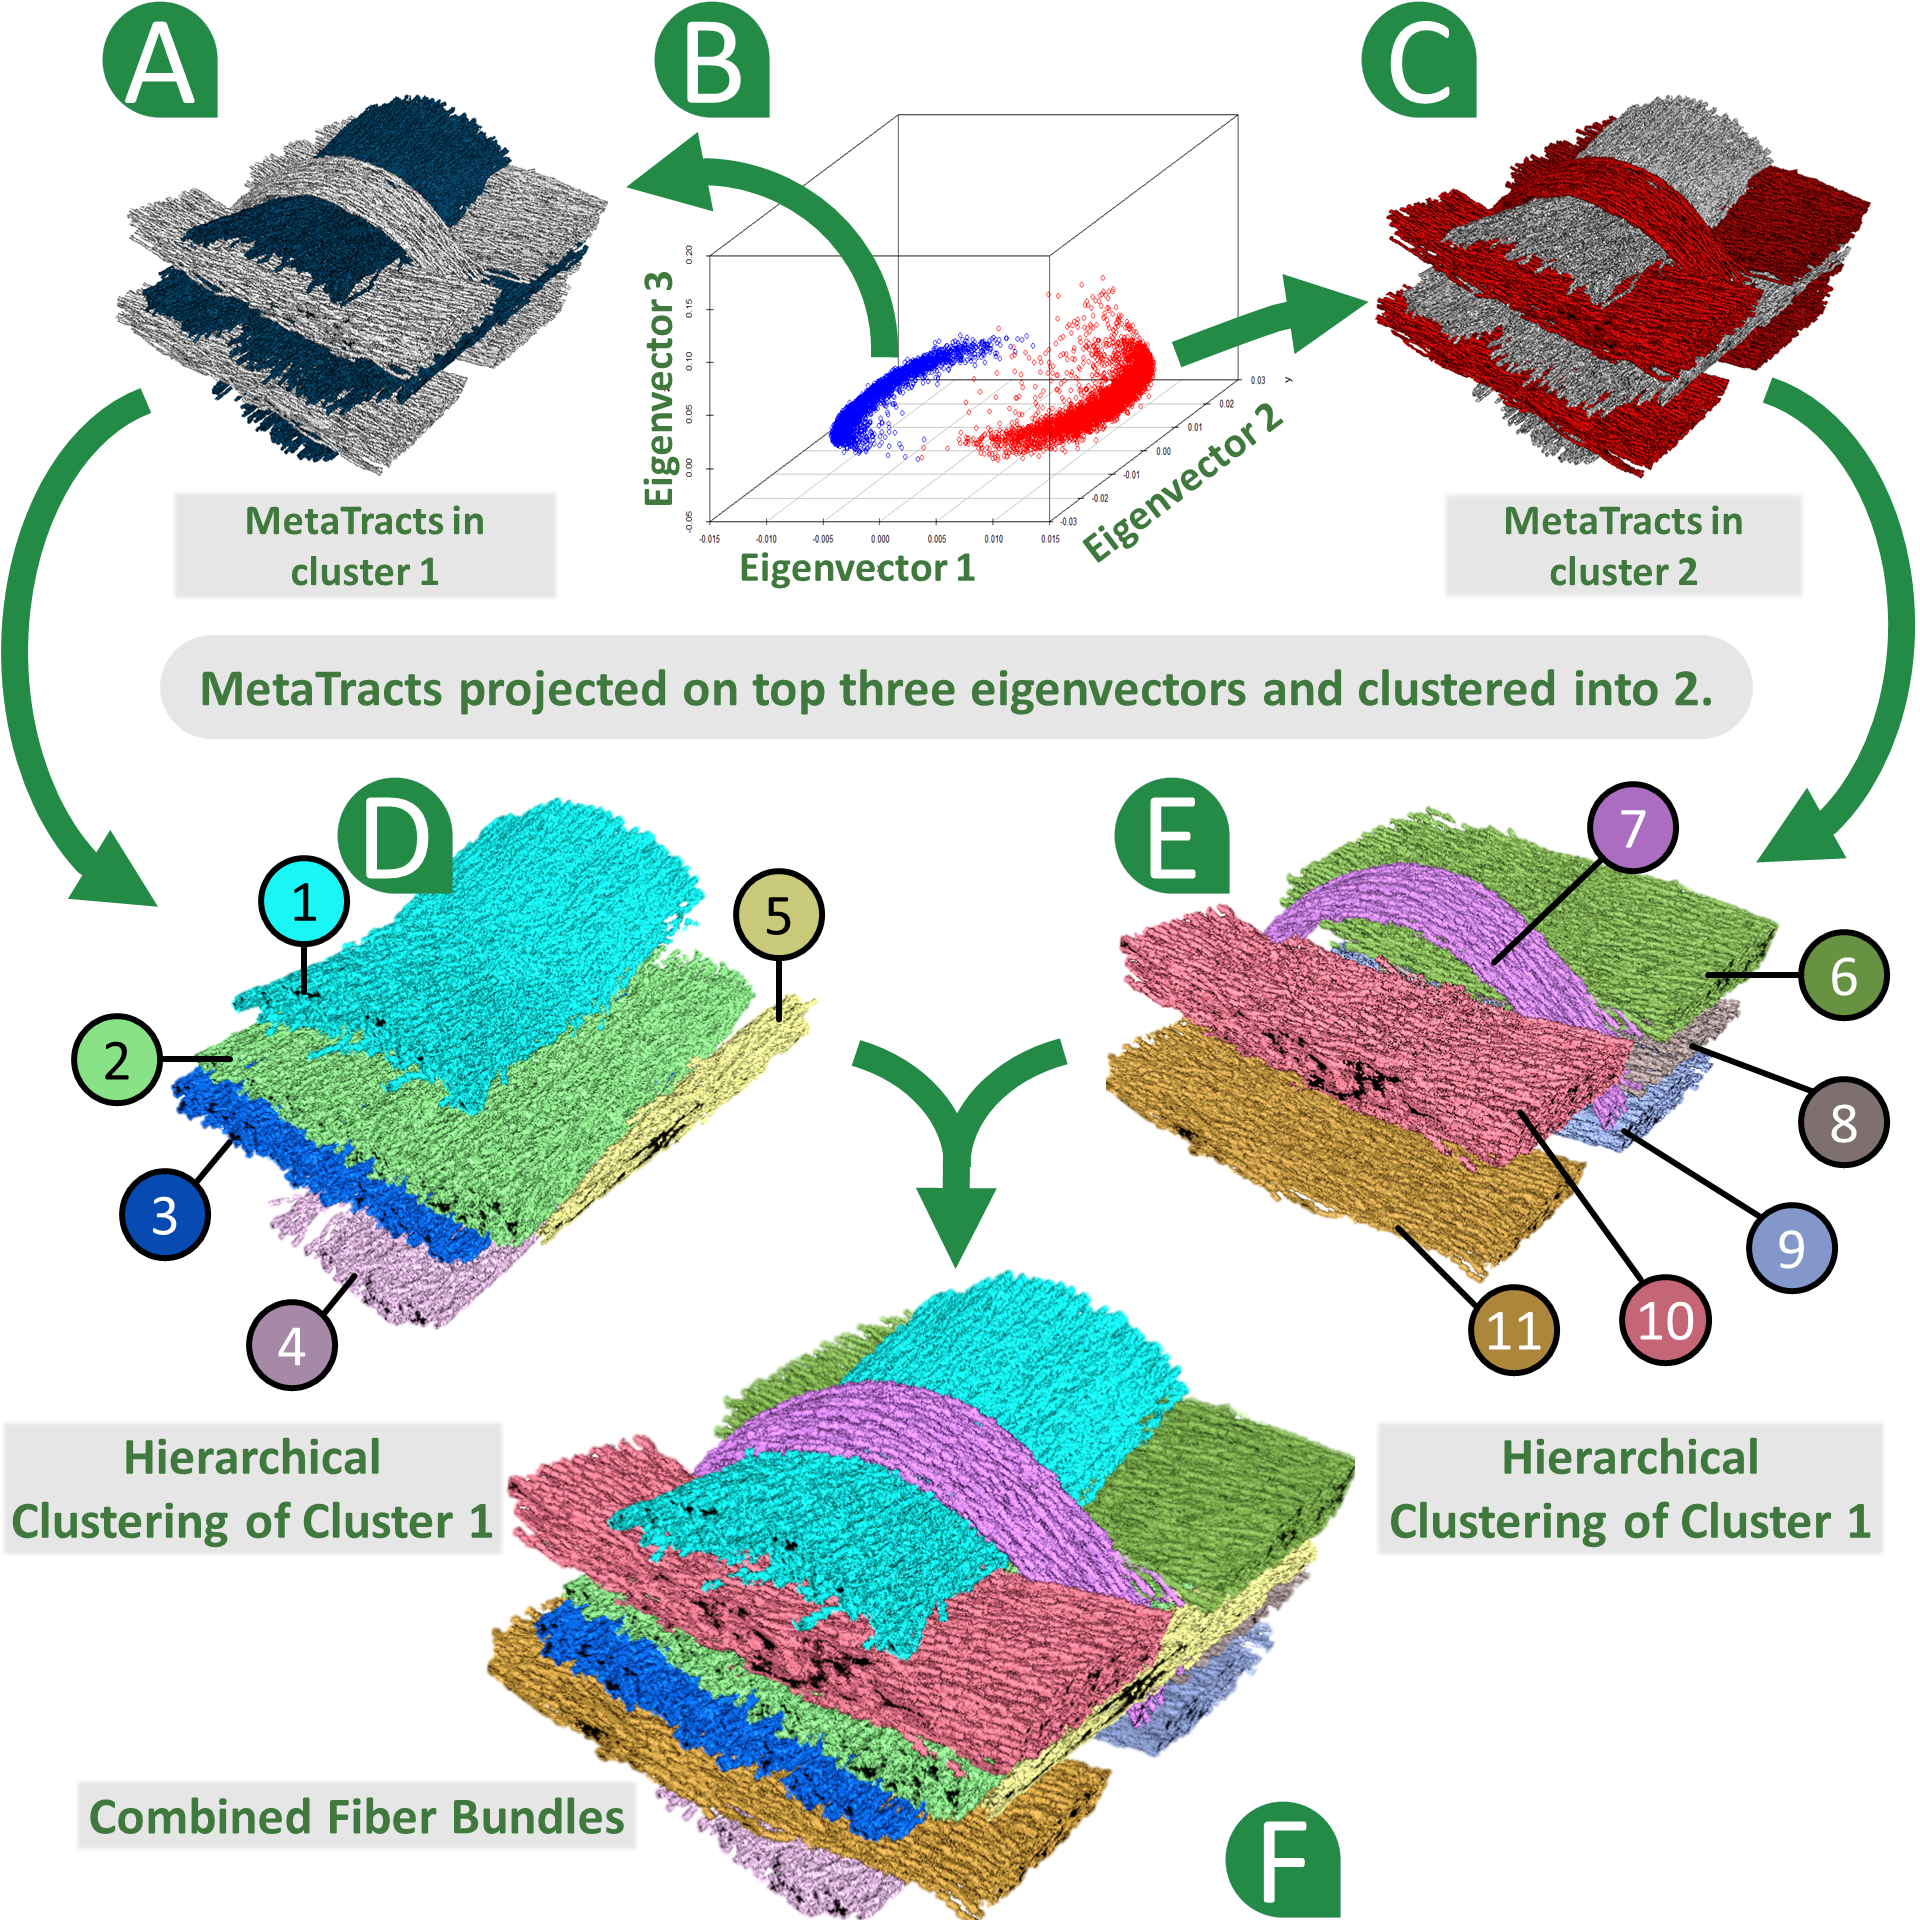
\includegraphics[width=0.45\textwidth]{imagesMT2014/image_clustering}
  	\caption{(B) Result of K means clustering with data points projected to the top three eigenvectors as major axes. (A) MetaTracts belonging to orientation cluster 1. (C) MetaTracts belonging to orientation cluster 2. MetaTracts in gray(A,C) show context.
  	(D,E) shows the result of distance based clustering on the orientation cluster. (F) shows the combined result. }
  \label{fig:orientation_clustering}
  \end{figure}

%\subsection {Distance based clustering}
%\label{subsec:dist_clustering}
%We now apply "single-linkage" hierarchical clustering~\cite{Moberts2005} to the results of the orientation clustering results.
%If we assume each fiber is represented as a set of points($C_P$) then the distance between two MetaTracts is computed as the minimum of the directed Hausdorff (maximum of the minimum euclidean) distances between points on the MetaTracts. Hierarchical clustering has one parameter, which is the number of clusters (h). Single linkage clustering inspite of it's advantages and  wide spread use, though suffers acutely in the presence of outliers.
%
%\begin{figure}[h]
%  \centering
%  	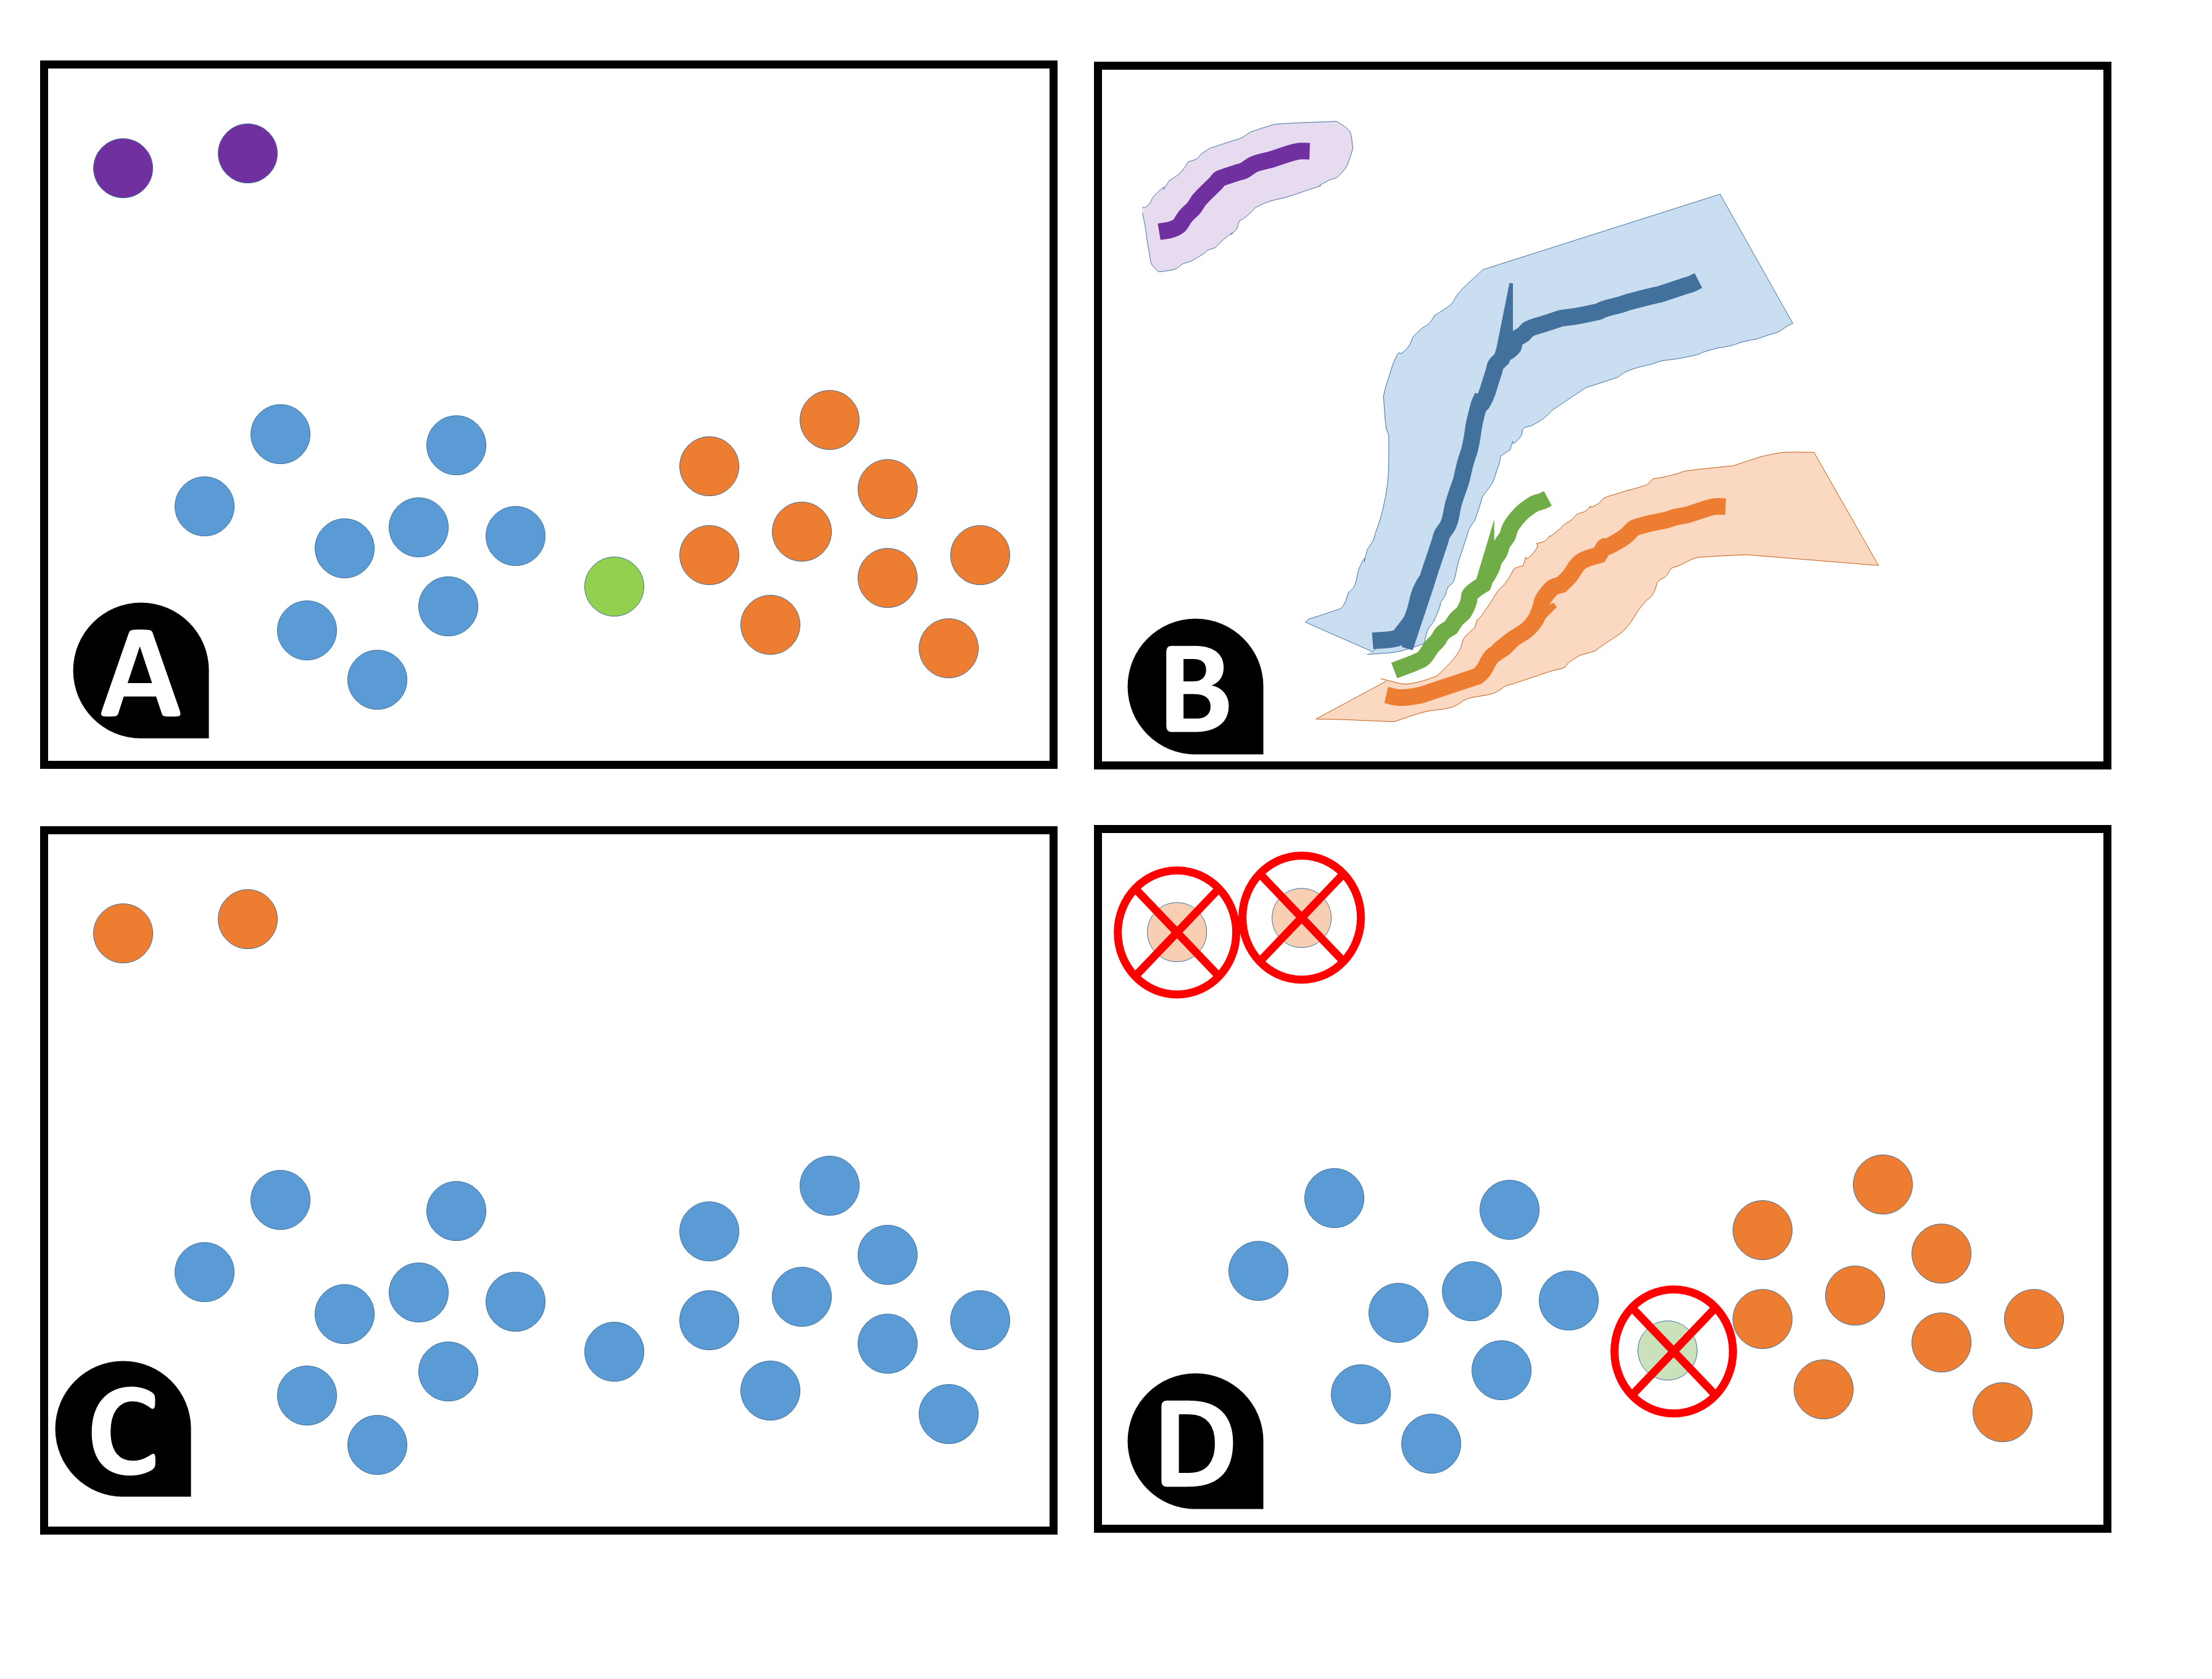
\includegraphics[ trim = 2cm 2cm 2cm 2cm, clip=true, width=0.3\textwidth]{imagesMT2014/clustering_probs_B.png}
%  	\caption{test}
%  \label{fig:cluster_prob_B}
%  \end{figure}
%For example Figure~\ref{fig:cluster_prob_B}B shows two main bundles (blue, orange), one outlier which has close proximity to both bundles (green) and another outlier far away from both the bundles (purple).
%Figure~\ref{fig:cluster_prob_B}A shows some sample MetaTracts from the bundles as points in a euclidean space.
%Setting h to 2 and performing single linkage hierarchical clustering would give a wrong result (Figure~\ref{fig:cluster_prob_B}C) It would create the outlier as a separate class instead of breaking the larger group. As a robust solution to the problem we perform hierarchical clustering iteratively. At each step removing clusters which have low cardinality(this is a common practice). However, we also remove elements from each cluster which have length lower than the median length of the fibers in the bundle. After a few iterations a stable state is reached where the outliers are removed and the clustering into bundles is robust(Figure~\ref{fig:cluster_prob_B}D).
%\begin{figure}[h]
%  \centering
%  	\includegraphics[ trim = 1cm 1cm 1cm 1cm, clip=true, width=0.3\textwidth]{imagesMT2014/final_clustering_A.png}
%  	\caption{Results of MetaTracts clustering. A: shows the X orientation cluster, clustered into 10 clusters. B: shows the Z orientation cluster, clustered into 10 clusters. Clusters with cardinality less than 10 are not shown. C: shows a close of the curved bundle extracted from the data. D: shows the original data for comparison.}
%  \label{fig:cluster_final_A}
%  \end{figure}
%  Figure~\ref{fig:cluster_final_A}(A,B) show the results of clustering each orientation bundle into ten clusters. Clusters with cardinality less than ten are not shown. Figure~\ref{fig:cluster_final_A}C shows the closeup of the curved bundle and Figure~\ref{fig:cluster_final_A}D shows the original data for reference. Single linkage clustering is very robust to the over-estimation of "h". A very large value of "h" would still keep the main clusters intact and create smaller  clusters with low cardinality which qualitatively does not degrade the results at all.

  
\subsection{Distance based clustering}
 \label{subsec:dist_clustering}
Orientation clustering uses only orientation information. To subdivide the oriented clusters into fiber bundles, we need to include further information about the geometric proximity between MetaTracts. We use the directed Hausdorff distance for distance based clustering.
Each MetaTract is represented as a set of points ($C_P$). Formally, the directed Hausdorff distance from point set P to point set Q is defined as 
$H_{dir}(P,Q) = max_{p \in P} min_{q \in Q} d(p,q)$ .
The Hausdorff distance is defined as $H(P,Q) = max(H_{dir}(P,Q),H_{dir}(Q,P))$.
The Hausdorff distance is a metric so $H(P,Q) \le H(P,Q') + H(Q',Q)$ but the directed Hausdorff is not.
Unfortunately, the Hausdorff distance does not work well for our application since a fiber bundle may have many MetaTract which only partially covers the bundle (Figure~\ref{fig:length_distribution}(B)). If a MetaTract $P$ covers only part of the fiber bundle covered by $Q$, then $H_{dir}(P,Q)$ will be very small while $H_{dir}(Q,P)$ will be large.
Thus, $H(P,Q)$ will be large, even though $P$ and $Q$ are in the same fiber bundle.
Instead of using the Hausdorff distance, $\max(H_{dir}(P,Q),H_{dir}(Q,P)$, we use $\min(H_{dir}(P,Q),H_{dir}(Q,P))$. If $P$ covers only part of the fiber bundle covered by $Q$, then $\min(H_{dir}(P,Q),H_{dir}(Q,P))$ is very small.
Note that if $P$ and $Q$ overlap but do not cover the same parts of the fiber bundle, then $H_{dir}(P,Q)$ and $H_{dir}(Q,P)$ and $\min(H_{dir}(P,Q),H_{dir}(Q,P))$ will be large.
 
The directed Hausdorff distance is very sensitive to outliers in the data.
However, because MetaTracts after orientation clustering are constructed using cylinders with similar orientations, they are not plagued by outliers.
To cluster based on MetaTract proximity, we used single linkage hierarchical clustering.
Hierarchical clustering has a single parameter $h$, the desired number of clusters.
In hierarchical clustering each objects starts in its own cluster and clusters are merged based on some criterion.
Clusters are merged until there are only $h$ clusters left.
Hierarchical clustering is intuitive since it is easy to trace how clusters are formed and merged.
Single linkage clustering finds pairs of objects $p \in P$ and $q \in Q$ where $P \neq Q$ which are closer than other such pairs, and merges the containing clusters $P$ and $Q$.
We found that single linkage hierarchical clustering had two major drawbacks.
First, the clustering would produce some small clusters of just a few MetaTracts.
These MetaTracts were anomalies caused by noise in the data and did not represent true fiber bundles.
Second, if two fiber bundles were parallel for some of their length and then separated, they would sometimes be clustered into the same fiber bundle.
A short MetaTract which was parallel to both and did not extend into the separation region could form a link between the two fiber bundles, causing them to be clustered into a single bundle.
To address the problem of small clusters, we applied hierarchical clustering and then identified small clusters with few MetaTracts.
We removed the MetaTracts that were in those clusters from the data set and reapplied hierarchical clustering.
To address the problem of short MetaTracts joining different fiber bundles, we applied hierarchical clustering and then removed the
shortest fibers (fibers less than 0.6 times the median length) in each bundle. We then reapplied hierarchical clustering.
We repeated both until a steady state of clusters is reached and no new small fibers can be removed. The results of clustering the orientation clusters Fig.~\ref{fig:orientation_clustering}(A,C) are shown in Fig.~\ref{fig:orientation_clustering}(D,E) respectively. Note how the purple cluster Fig.~\ref{fig:orientation_clustering}(E) bundle ``7'' is extracted well.
\begin{figure}
\centering
		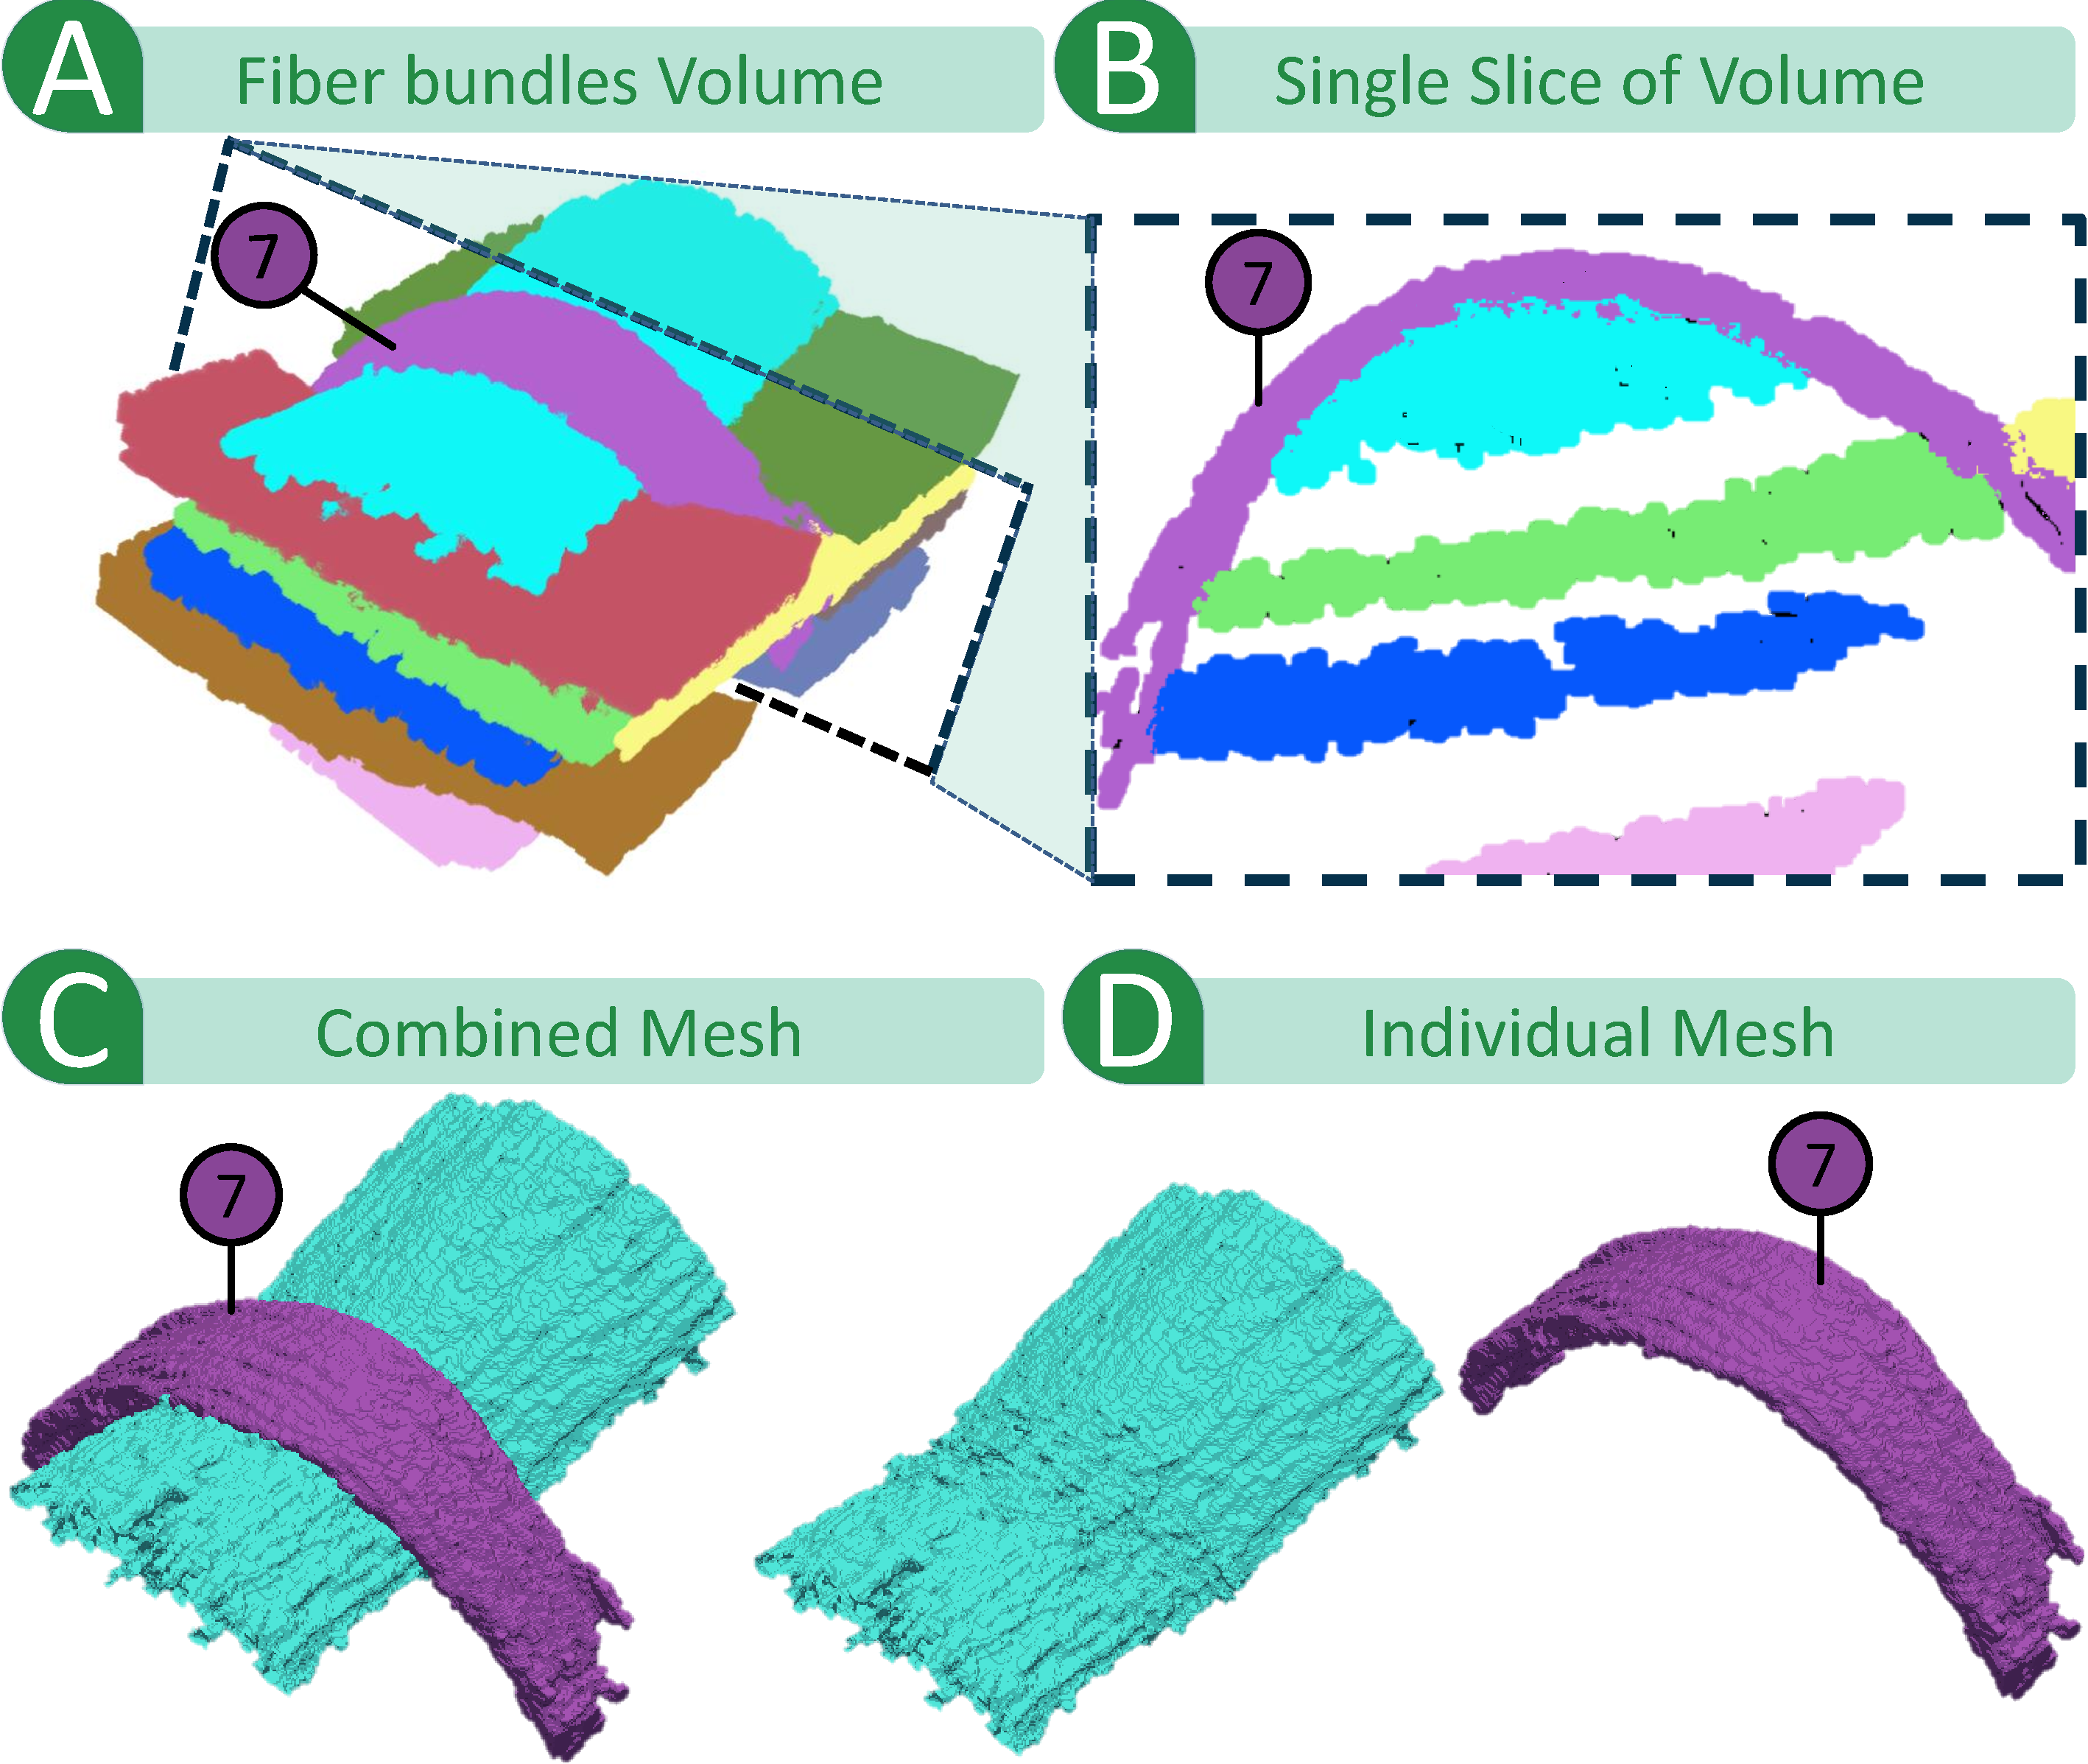
\includegraphics[width=0.4\textwidth]{images_pvis/figure7}
		%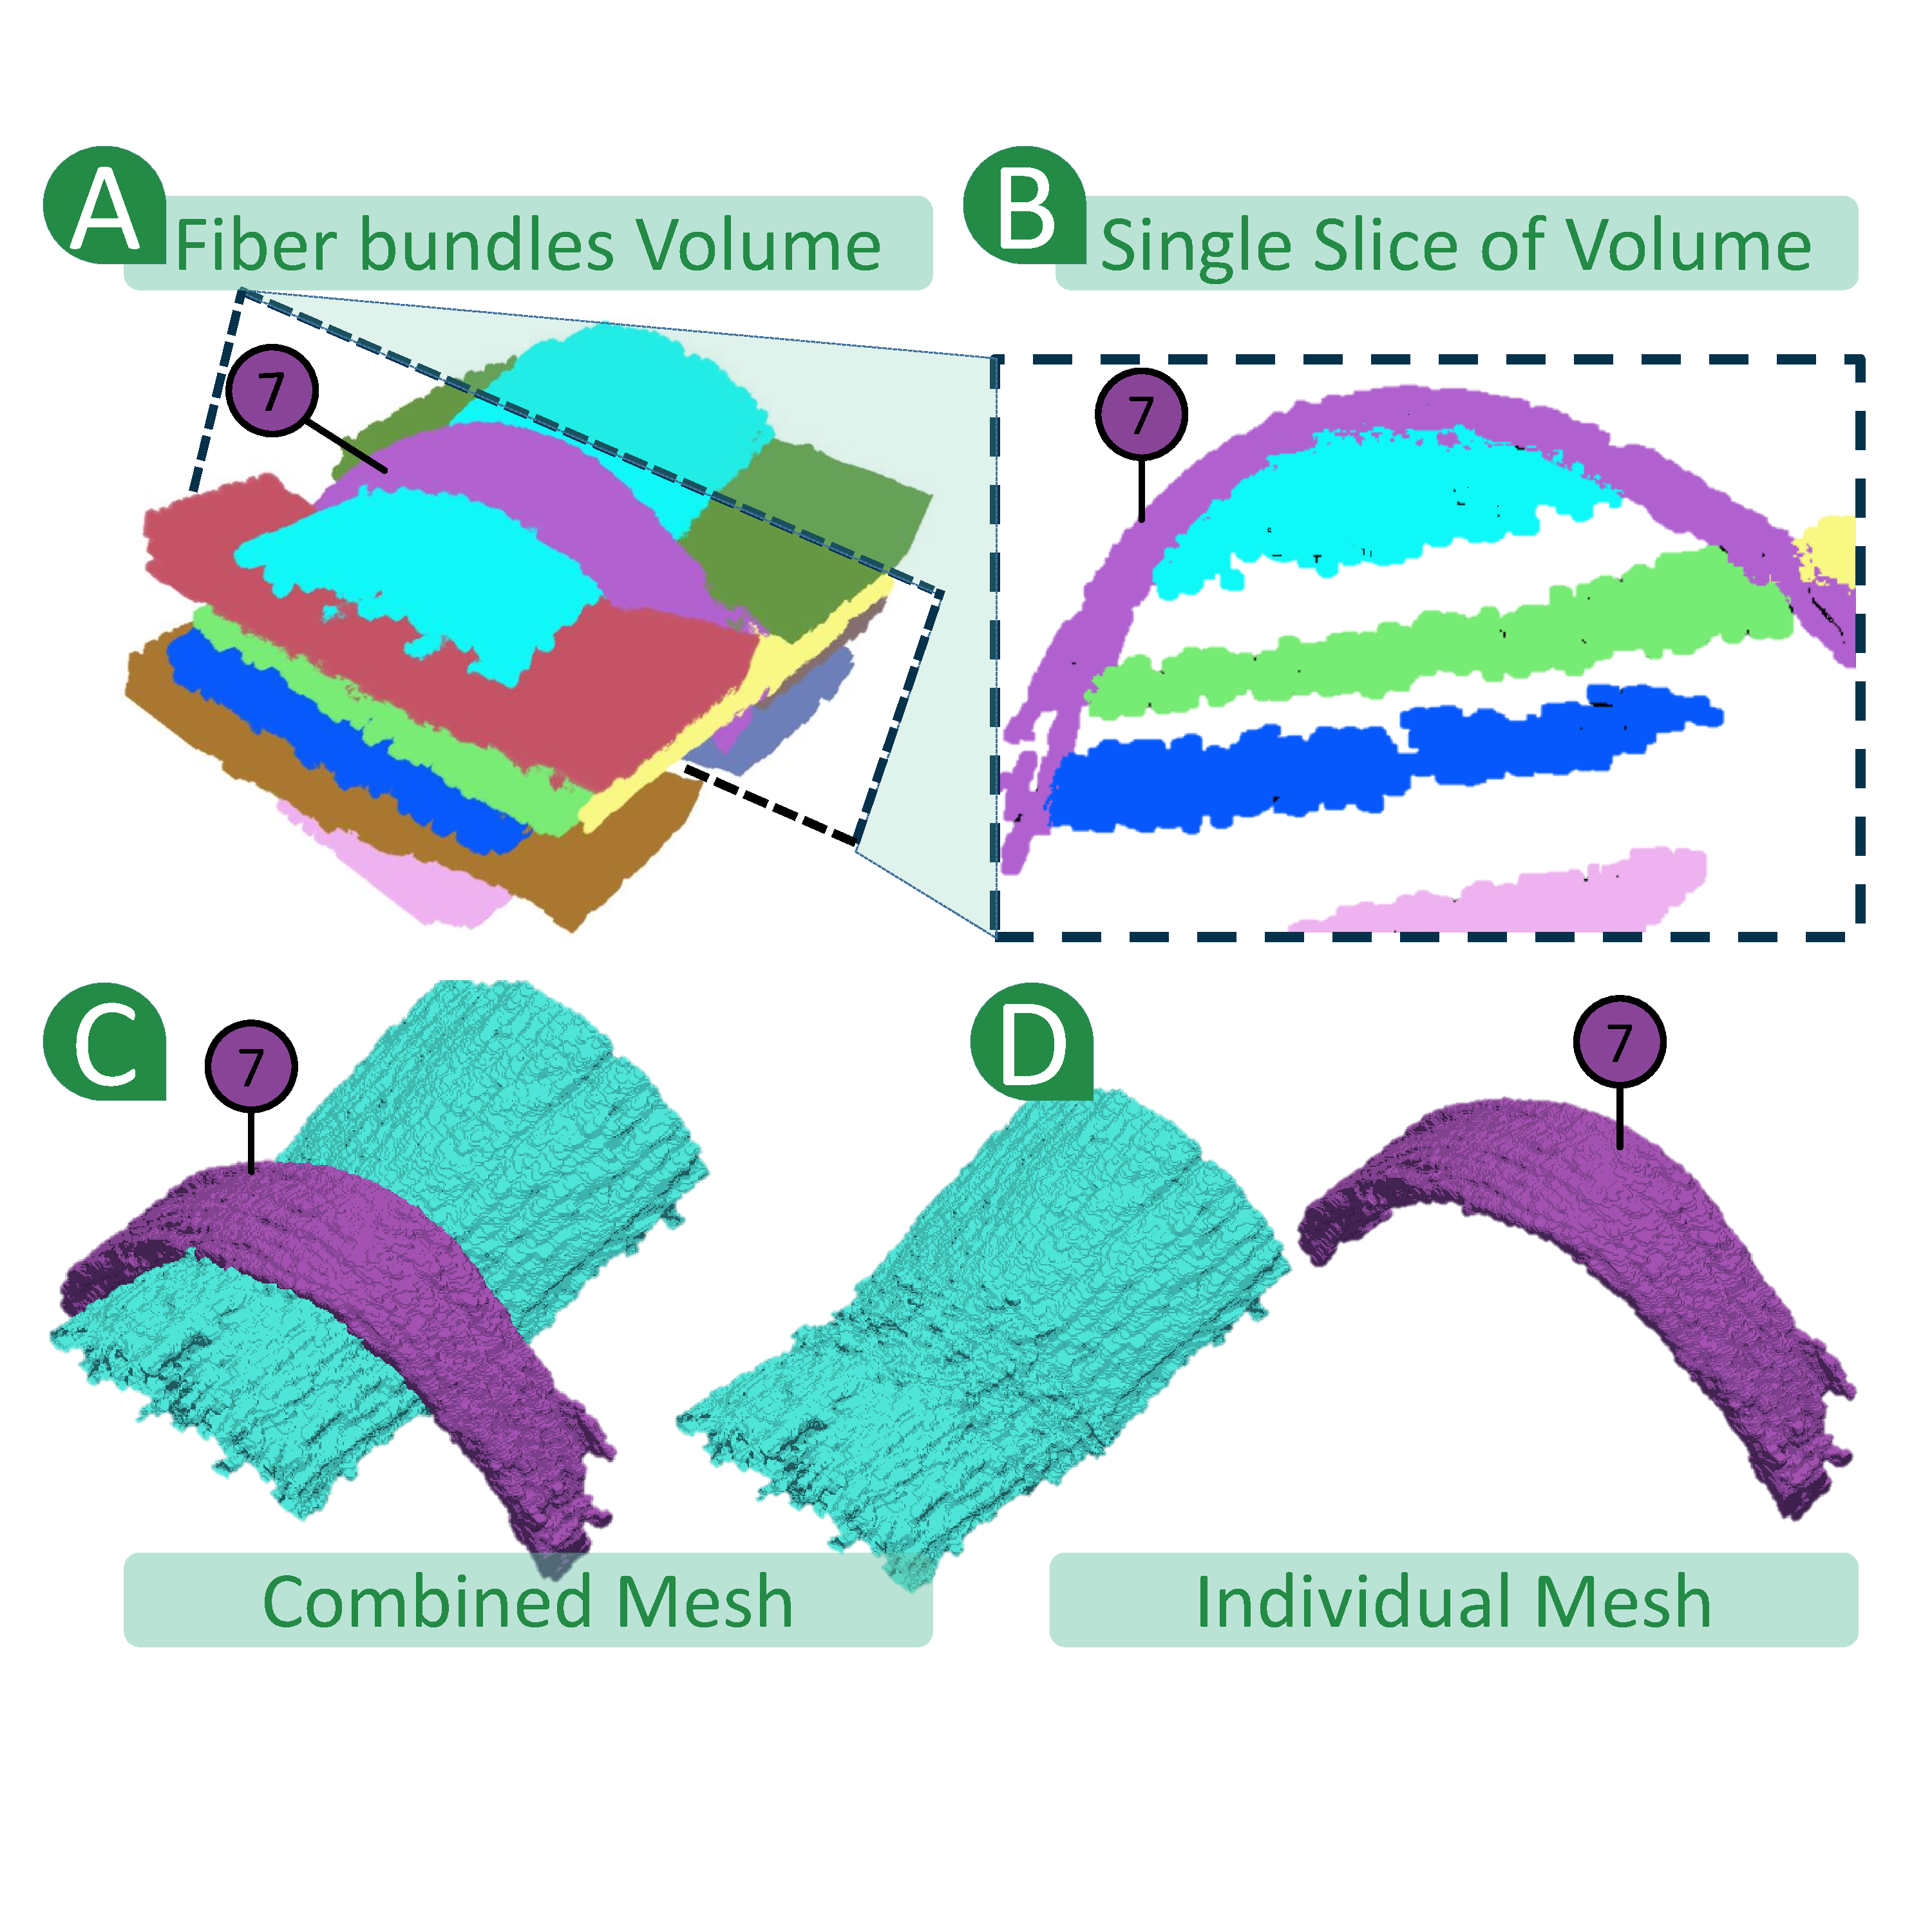
\includegraphics[width=0.5\textwidth, trim = 0mm 70mm 0mm 20mm, clip]{imagesMT2014/image7b.pdf}
	%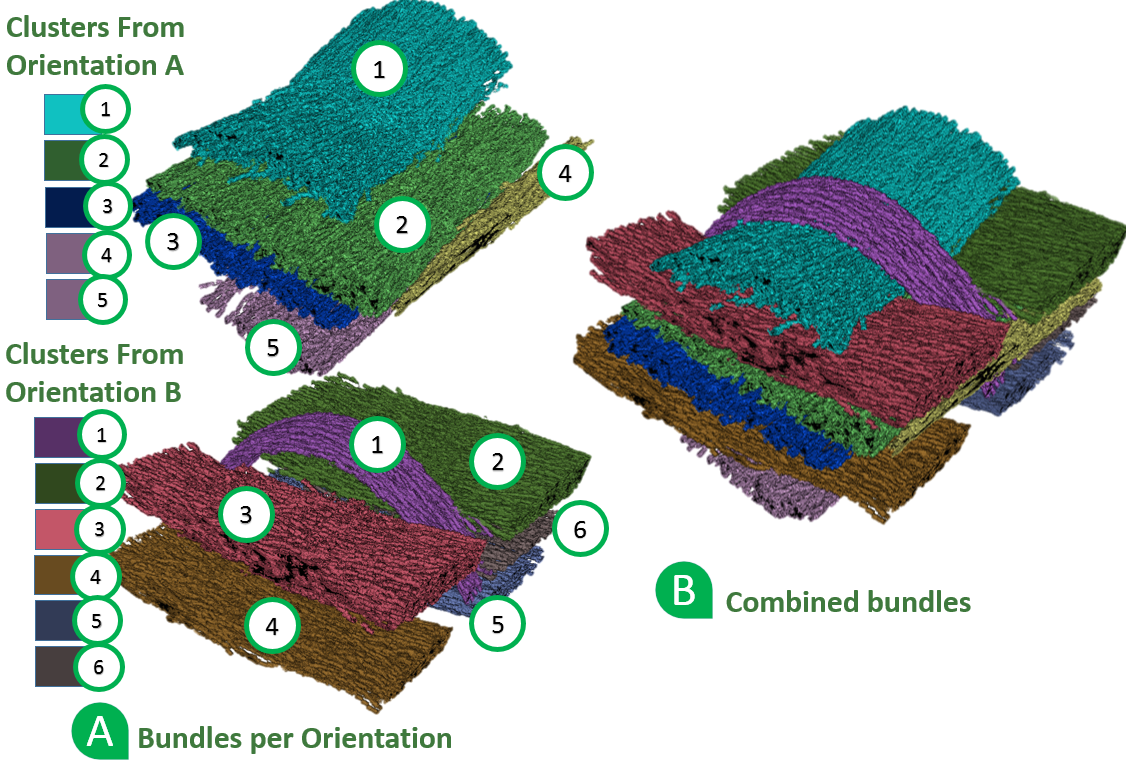
\includegraphics[width=0.45\textwidth]{imagesMT2014/crop-16/bundles}~ 
	%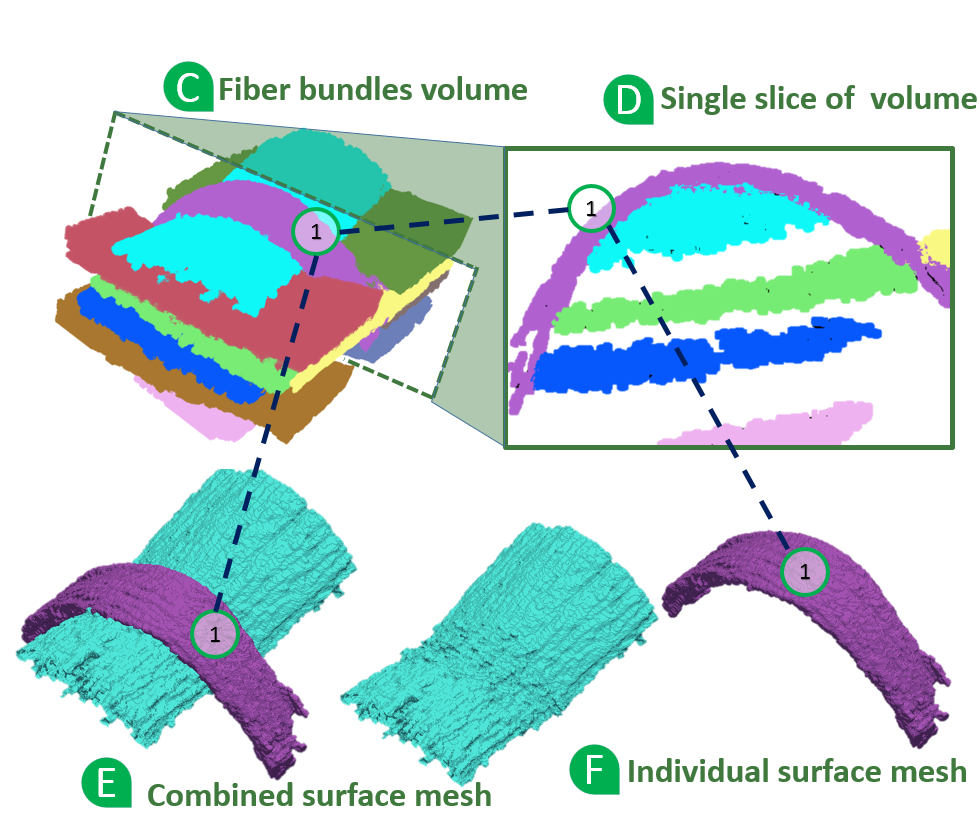
\includegraphics[height=0.35\textwidth]{imagesMT2014/crop-16/vol_mesh.png} 
	\caption{(A) Volume rendering of data set Figure~\ref{fig:data-char}A.(B) shows a single slice of the data set. (C) shows two of the extracted meshes together. (D) shows the meshes separately.}
	\label{fig:crop-16-decomp}
\end{figure}  
  
  
% We in our approach use Zhang et al.~\cite{Zhang2008} Hierarchical clustering approach. Zhang et al.\cite{Zhang2008} define the distance between two DTI fibers Q and R as the larger mean of thresholded closest distances (equation \ref{eqn:dist}).
%In the above discussion,DTI fibers are represented as points in $\mathbb{R}^3$. MetaTracts can be correspondingly represented as points in  $\mathbb{R}^3$ in terms of the start points of the cylinders. In our implementation Q and R are sets of `$C_{p}$'s. We in our implementation set $t$ to be same radius of the cylinders for all our tests. If two MetaTracts are less than a width of the cylinder apart then they are describing the same region. We use $D_{Lt}$ as our proximity measure.
%\begin{equation}\label{eqn:dist}
%D_{Lt}(Q,R,t)= max (d_{t}(Q,R,t),d_{t}(R,Q,t))
%\end{equation} 
%where, 
%\begin{equation}\label{eqn:dist-2}
%d_{t}(Q,R,t)= mean_{a\in Q,(min_{b\in R})\parallel a-b\parallel \geq t } min_{b\in R}
%{\parallel a-b\parallel}
%\end{equation} 
%The input to this step are the results of orientation based clustering (fig.~\ref{fig:clustering}b), the figure along with our data assumptions  provides some reasoning why $D_{Lt}$ is effective in our case. The MetaTracts donot necessarily run from boundary to boundary of our data. In fig.~\ref{fig:clustering}b, "Orange", MetaTracts within the  yellow rectangle might be "diverging" (running parallel for a distance and then diverge~\cite{Zhang2008}). Also, while the MetaTracts are close at some points, they belong to different bundles. So unlike the orientation measure,  mean of closest distance $d_{t}(Q,R,t)$ is a better fit than single point comparison.
%
%Hierarchical clustering approaches have one main parameter, which is the number of clusters $h$. For each cluster extracted based on the orientation phase we cluster the result into $h$ clusters. Fig. \ref{fig:clustering} (c) shows the result from hierarchical clustering.
%
%\subsection {Notes on Clustering techniques}
%\label{subsec:other_clustering}
% The current two phase clustering technique was chosen for its simplicity, relevance to the domain understanding, intuitive nature of the parameters ($K$ and $h$, see sec~\ref{sec:param_choices}). Moberts et al.~\cite{Moberts2005} also remarks that specifying number of clusters is more intuitive than other criterias such as  number of neighbors and edge thresholds. Secondly, on average we have around ten thousand individual tracts. Solving the eigen decomposition problem for such large number of tracts in time consuming. Once the orientation clustering is completed, for each particular orientation the number of fibers being compared in less, and  hierarchical  clustering can be done in a fraction of time compared to the eigen based approach this makes the choosing of $h$ an interactive process. 


\section {Voxelization and surface extraction}
\label{sec:vis}
Apart from direct visualization of the MetaTracts, we show two simple yet highly important extensions for our domain specialist. The first one is to voxelize the original volume according to the clusters each voxel is associated with.
The second is to extract the corresponding surfaces from the voxel data by binarizing the volume per cluster and extracting the isosurface of the largest connected component from the binary volume. Both methods can possibly be used for further analysis of the data, e.g. in simulations.
To voxelize the space,  we compute a neighborhood around each voxel. We then enumerate the number of voxels of each class (cluster) in this neighborhood. The voxel is then assigned to the class with the maximum number of elements in the neighborhood. Figure~\ref{fig:crop-16-decomp}A and Figure~\ref{fig:prepreg}D shows the result of voxelization. Figure~\ref{fig:crop-16-decomp}(C, D) show examples of extracted meshes.
%The MetaTracts and the clustering provide an abstraction of the fiber bundles and are used as a visualization tool. Through visualization MetaTracts we can answer all the queries mentioned in Section~\ref{sec:intro}. 
%
%In this Section we show two simple extensions to the MetaTracts and discuss how the end user might benefit from each. One way to visualize  the bundles is to color map the original volume according to the clusters each voxels are associated with (Section~\ref{subsec:voxel}). The second is to extract the surfaces from the voxel data (Section~\ref{subsec:surf_ext}). The visualizations can be used together, for example Fig.~\ref{fig:crop-13-mesh}e shows the crossover bundle as a mesh overlay on the MetaTracts.
%
%\subsection{Voxelization}
%\label{subsec:voxel}
%
%We take the following approach for associating a voxel $v$ with one of the cluster classes. We compute a neighborhood around each voxel. We enumerate the number of voxels of each class in this neighborhood. The voxel $v$ is then assigned to the class with the maximum number of elements inside the neighborhood. In this particular implementation, we look for neighbors in a ball of radius $r$ around the voxel. Intuitively  this is a modification of the flood-fill algorithm. In practice, we observed that a suitable value of the radius is half the distance used for seeding the volume.
%More sophisticated approaches could be employed depending upon the error-tolerance of the application used. Fig.~\ref{fig:crop-13-mesh}a shows the results of applying the voxelization step to the clustering result shown in Fig.~\ref{fig:clustering}c. This adds a level of abstraction over the MetaTracts visualization and brings us closer to the declared goal of visualizing the bundles directly at individual voxel level. Clipping planes through the voxel data can then clearly show the changing sizes of cross-sections of the bundles.
%
%\begin{figure}
%  \centering
%   \subfloat[]{\includegraphics[width=0.2\linewidth]{imagesMetaTracts/crop-13voxel.eps}}
%  \subfloat[]{\includegraphics[width=0.22\linewidth]{imagesMetaTracts/crop-13-mesh-b.eps}}
%  \subfloat[]{\includegraphics[width=0.18\linewidth]{imagesMetaTracts/crop-13-mesh-a.eps}}
%  \subfloat[]{\includegraphics[width=0.21\linewidth]{imagesMetaTracts/crop-13-mesh-c.eps}}
%  \subfloat[]{\includegraphics[width=0.24\linewidth]{imagesMetaTracts/mtSurf-2}}
%  \caption{Visualization: (a) shows the voxelization. (b) shows the result of extracting surfaces from the result of the voxelization step (Clusters with very few elements have been discarded as a post processing step.), (c) and (d) shows the clusters in particular orientation direction.(e)shows the cross-over bundle as a mesh overlay on the MetaTracts. }\label{fig:crop-13-mesh}
%\end{figure}
%
%
%\subsection{Surface Extraction}
%\label{subsec:surf_ext}
%The voxelization step divides the image volume into coherent clusters. Where each voxel is associated with the cluster index of the corresponding fiber bundles. We can then use isosurfacing algorithms to find the boundaries of separation of the clustered classes. This step produces a triangular mesh following the popular marching cubes algorithm \cite{Lorensen1987}. The surfaces are computed for each of the clusters based on the voxelized grid. Our rather simple voxelization criterion means we cannot guarantee any convex or manifold criteria without adopting a more sophisticated material boundary separation algorithm.
%
%In a post processing step we remove clusters whose number of elements are far less than the mean number of elements per cluster. This simply removes outliers generated by the hierarchical clustering of classes with very few members. Fig.~\ref{fig:crop-13-mesh} shows the results of surface extraction. Fig.~\ref{fig:crop-13-mesh}b shows all the triangle meshes. Fig.~\ref{fig:crop-13-mesh}c and Fig.~\ref{fig:crop-13-mesh}d shows the meshes from two different orientation clusters. 
%Fig.~\ref{fig:crop-6} shows more results. Further processing techniques such as finding the medial axis might be applied to the extracted surface. Other NDT methods which takes meshes as input can also be utilized.


\section {Experimental Results}
\label {sec:results}
%\begin{figure*}
%\centering
%\captionsetup[subfigure]{labelformat=empty}
%	%\subfloat[]{\includegraphics[width=0.10\textwidth]{imagesMT2014/crop-6-G.PNG}}
%	%\subfloat[]{\includegraphics[width=0.10\textwidth]{imagesMT2014/crop-6-H.PNG}}
%	%\subfloat[]{\includegraphics[width=0.35\textwidth]{imagesMT2014/crop-6-I.PNG}}
%	
%	\subfloat[(a) Dat set 2]{\includegraphics[width=0.7\linewidth]{imagesMT2014/prepreg/Capture8.PNG}}
%	\subfloat[(b) Data set 3]{\includegraphics[width=0.2\linewidth]{imagesMT2014/dataset203.png}}	
%	\caption{(a) Shows in order, the volume rendering of the second data set, a single (2D) slice, the orientation clustering bundles and the final bundles followed by proximity clustering. (b) Shows in order the third data set, a single (2D) slice and finally the extracted fiber bundles.}
%	\label{fig:crop-6}
%\end{figure*}

\begin{figure}[t]
\centering
	%\includegraphics[width=0.45\textwidth]{imagesMT2014/image8b}
	\includegraphics[width=0.4\textwidth, trim = 0mm 30mm 0mm 0mm, clip,]{images_pvis/figure8}
	\caption{Data set with flat thin and compact bundles. (A) shows the volume rendering and a 2D slice with one of the boundaries marked in green, (B) shows the clusters according to individual orientation. (C) shows the complete result. (D) shows the voxelization of (C).}
	\label{fig:prepreg}
\end{figure}

%Fig~\ref{fig:kull} (b) shows the results after the MetaTracts extraction. Fig.~\ref{fig:kull} (c) shows the results of the orientation clustering with $K$ set to 2. Note, that the curved fiber bundle has also been detected with the correct orientation. Fig. \ref{fig:kull} (d) and (e) shows the results of hierarchical clustering of \ref{fig:kull} (c) using proximity based clustering. Both the orientation were clustered into 14 classes.

 %glass
We tested our method on multiple datasets with varying characteristics. 
Figure~\ref{fig:orientation_clustering} shows the result of data set~\ref{fig:data-char} decomposed into 2 orientation and each orientation decomposed into 10 clusters (the ground truth is 6 and 5 respectively). The hierarchical clustering is robust to over segmentation.
Figure~\ref{fig:len_dist_crop16} shows the median, minimum and maximum lengths per cluster. We generate the correct clusters and outlier bundles with very few elements which can be discarded. As noted in section~\ref{subsec:dist_clustering} the tracts do not run the entire length of the dataset, the median length of MetaTracts in cluster 6 Fig.~\ref{fig:length_distribution} is 200 while the maximum MetaTract in the bundle is about 500 (measured in units of grid cube length). Fig.~\ref{fig:length_distribution}(B) shows the length per MetaTract distribution for a particular fiber bundle. 
Fig.~\ref{fig:prepreg} shows the results on our dataset2. This dataset is dense with \textit{flat and thin} bundles. The dimensions are 300x350x300 and the datatype is uint16 (compared to dataset1 which was only uint8). The bundles are indistinguishable in the original data set Fig.~\ref{fig:prepreg}(A). A green dotted line shows one of the fiber bundle boundary. Fig.~\ref{fig:prepreg}(B) shows the fiber bundles for the two orientation. Fig.~\ref{fig:prepreg}(C) shows the combined results.Fig.~\ref{fig:prepreg}(D) shows the volume after voxelization.
The fiber bundle extraction using MetaTracts was implemented in C++ using ITK. All clustering was done in R. The preprocessing consists of MetaTract generation the distance computation and the orientation clustering. The hierarchical clustering separately, on the results of the orientation clusters can be done quickly in a few minutes on a Intel Xeon E5-2667 workstation according to user input `h'(section~\ref{sec:param_choices}). We store the normalized direction at each fiber point, thus both distance measures can be extracted simultaneously without extra computation.


\section {User Evaluation}
\label {sec:user_eval}
We integrated MetaTracts into a tool and created a user evaluation questionnaire which we distributed.
%\begin{figure}[h]
%\centering
%\subfloat[]{\includegraphics[width=0.25\textwidth]{imagesMT2014/crop-6-F.PNG}}
%\subfloat[]{\includegraphics[width=0.25\textwidth]{imagesMT2014/orientB.PNG}}
%\caption{Contextual information: (a) Shows the four largest clusters in the data set in Fig~\ref{fig:prepreg}.
%(b) shows how the red bundle `bends' under the green bundle, which is not immediately apparent from just the volume rendering.}
%\label{fig:context}
%\end{figure}


\section{Parameter choices}
\label{sec:param_choices}
\begin{figure}
\centering
	\includegraphics[width=0.5\textwidth,  trim = 0mm 260mm 0mm 15mm, clip]{images_pvis/figure9}
	%\includegraphics[width=0.5\textwidth,  trim = 10mm 40mm 0mm 15mm, clip]{imagesMT2014/image_length_histogram.pdf}
	\caption{Number of tracts and median, minimum and maximum length of individual MetaTracts in the orientation cluster Fig.~\ref{fig:orientation_clustering}, clustered into 10 clusters (Fig.~\ref{fig:crop-16-decomp}A top). The unit for length is the grid cube length. Figure~\ref{fig:length_distribution}(B) shows the length of individual MetaTracts in cluster 6. Clusters labeled 2,3,4,5 and 7 all have cardinality less than 10. }
	\label{fig:len_dist_crop16}
\end{figure}
The critical parameters are $K$ for the K-means in orientation based clustering and $h$ for the hierarchical clustering. K denotes the number of major directions, which is either known a priori or can be easily estimated by looking at the weaving pattern. 
Our framework is robust to the choice of $h$ (Section~\ref{sec:results}). Large $h$ keeps the major bundles intact. For example, in  Fig.~\ref{fig:len_dist_crop16}, where $h$ was set to ten while the ground truth was five, we observe that the major clusters remain well segmented and small clusters can be removed if they have too few elements (clusters 2,3,4,5 and 7 in Fig.~\ref{fig:len_dist_crop16} all have less than 10 elements). This is an appealing trait of the proximity based clustering, thus providing good results even when exact $h$ might be unknown.
The following parameters were fixed for all the tests. We set the reliable Hessian threshold $R_{h}$ to be 0.3 for all our tests. A $R_{h}$ of 0.0 would mean all points have reliable local orientation which would cause spurious MetaTracts detection. On the other hand a very high $ R_{h}$ would lead to be a decline in number of MetaTracts produced. The $\alpha$ and $\beta$ in $R_{h}$ are as explained in Frangi et al. \cite{Frangi1998} and set to 0.5. The length and the width parameters for the cylinders for the MetaTracts decide how coarse the fiber cylinders are. Larger cylinders will handle noisy local orientation better as it inspects a higher number of candidate points to extend the fiber. We used 10.00 and 2.00 for length and breadth, respectively for all tests. $\alpha$ and $\beta$ in equation~\ref{eqn:algo_1} decide how quickly the value of the factor decays, we have used [7-10] and half the length of cylinder (5.0). Our number of fiber bundle directions are limited, thus even for small $\eta$, the distinction between the orientation clusters is preserved quite well. We compared  $\eta=3-7$ experimentally without any dramatic change in results. 
%\begin{figure}
%\centering
% \subfloat[$\eta=7$]{\includegraphics[width=0.3\linewidth]{imagesMetaTracts/Rplot-ndim3k2}}
%  \subfloat[$\eta=3$]{\includegraphics[width=0.3\linewidth]{imagesMetaTracts/Rplot-ndim7k2}}
%  \caption{Embedding from $\mathbb{R}^m\to \mathbb{R}^\eta$, here m is the number of MetaTracts, 580 for this example. Followed by clustering into K=2 clusters.}
%  \label{fig:eta}
%\end{figure}
%\begin{figure}[htp]
%\centering
% \includegraphics[width=\linewidth]{imagesMetaTracts/kul-results.eps}
%  \caption{Results from orientation based dimensionality reduction and clustering. A is the original data set, B shows the results of fiber tracking. C shows the results of orientation based clustering and D shows the results of the proximity based clustering. }\label{fig:kull-full}
%\end{figure}

%\begin{figure}[htp]
%\centering
% \includegraphics[width=\linewidth]{imagesMetaTracts/glass-clus-2.eps}
%  \caption{ Fig  A and C shows the results fiber extraction. B and D shows the results of clustering with clipping planes.}\label{fig:closeup-full}
%\end{figure}


\section{Conclusion and future work}
\label{sec:conclusions}
In this paper, we introduce a framework to extract and visualize fiber bundles in composite materials. We show that our framework works at comparatively low resolution and with dense fiber arrangements (when extracting single fibers might not be possible). It handles complex fiber patterns such as ``cross overs'' and ``braiding''. The presented techniques are attractive and novel features for a industrial fiber bundle visualization tool.
%
%\begin{figure}
%  \centering
%  \subfloat[]{\includegraphics[width=0.2\linewidth]{imagesMetaTracts/crop-6-scalar.eps}}
%  \subfloat[]{\includegraphics[width=0.2\linewidth]{imagesMetaTracts/crop-6-tracks-1.eps}}
%  \subfloat[]{\includegraphics[width=0.2\linewidth]{imagesMetaTracts/crop-6-tracks-clus-a.eps}}
%    \subfloat[]{\includegraphics[width=0.2\linewidth]{imagesMetaTracts/crop-6-tracks-clus-b.eps}}
%  \subfloat[]{\includegraphics[width=0.2\linewidth]{imagesMetaTracts/crop-6-labels-all.eps}}
%  \caption{Dense data set with bundles which are flat and thin. (a) shows the results original dataset, (b) shows the results of metaTract extraction, (c) shows the results of our two step clustering  into 14 classes. (d) shows the results of voxelization  and (e) shows the results of surface extraction. }\label{fig:crop-6}
%\end{figure}
%% if specified like this the section will be ommitted in review mode


%\acknowledgements{
% The research leading to these results has received funding from the European Union’s Seventh Framework Programme (FP7/2007-2013) under grant agreement ACP2-GA-2012-314562-QUICOM. Our special thanks go to Ilya Ilya Straumit (KU Leuven) who provided us with dataset1.
%}




\bibliographystyle{abbrv}
%%use following if all content of bibtex file should be shown
%\nocite{*}
\bibliography{xBundle}
%\pagebreak
\clearpage
\section{Supplementary Material}
\label{sec:sm}
 In this section we show the results of some extended tests.
 section~\ref{subsec:glass} shows our results on glass fibers. Section~\ref{subsec:vox_ex} shows the some more results of voxelization and mesh generation. Section~\ref{subsec:compare} shows comparisons to hierarchical clustering and with individual fiber extraction technique. Finally, section~\ref{subsec:robustness} shows another result with different parameter to show robustness of parameter selection.
 
\begin{figure}
\centering
\subfloat[]{\includegraphics[width=0.25\linewidth]{imagesMT2014/glass-scalar.eps}}
  \subfloat[]{\includegraphics[width=0.25\linewidth]{imagesMT2014/glass-scalar-slice}}
  \subfloat[]{\includegraphics[width=0.25\linewidth]{imagesMT2014/glass-cluster-b.eps}}
  \subfloat[]{\includegraphics[width=0.25\linewidth]{imagesMT2014/glass-cluster-a.eps}}
  \caption{Our algorithm on a data set made of glass fibers. (a) The scalar dataset, (b) Depicts a slice from the data set, the  fibers are clearly demarcated from the rest of the matrix as oppose to the type of data  where it is hard to distinguish the fibers (Fig.~\ref{fig:data-char} or Fig.~\ref{fig:prepreg}A). (c) The result of the MetaTracts process, the colors are to help visualization. (d) The result of the orientation based clustering, the two clusters are marked red and yellow.}\label{fig:glass}
\end{figure}
\subsection{Glass Fibers}
\label{subsec:glass}
One simple way we used to validate the accuracy of shape and size of the extracted MetaTracts, is to run the MetaTract technique on Glass fibers.
Unlike the presented data, in glass the fibers are clearly visible (Fig.~\ref{fig:glass}(a)). We noted that the extracted MetaTracts closely followed the fibers in the data.
\subsection{Voxelization and surface extraction Extended}
\label{subsec:vox_ex}
The voxelization results and some of the meshes extracted from our second data set (Fig.~\ref{fig:prepreg}) are shown in Fig.~\ref{fig:vox_extended}.
\begin{figure}[h]
\centering
\subfloat[]{\includegraphics[width=0.2\textwidth]{imagesMT2014/crop-6-C2-vol}}
\subfloat[]{\includegraphics[width=0.2\textwidth]{imagesMT2014/mesh_prepreg_A}}
\\
\caption{(a) Voxelization of Fig.~\ref{fig:prepreg}C, (b) Shows some of the extracted meshes.}
\label{fig:vox_extended}
\end{figure}
\begin{figure}[h]
\centering
\includegraphics[width=0.5\textwidth]{imagesMT2014/UserStudy/vol_crop16}
\\
\caption{ A shows the Voxelization of Fig.~\ref{fig:data-char}. B shows a single slice. C the slice of original data. }
\label{fig:vox_extended_crop16}
\end{figure}

\begin{figure}[h]
\centering
\subfloat[]{\includegraphics[width=0.25\linewidth]{imagesMT2014/compare-clus-1.eps}}
\subfloat[]{\includegraphics[width=0.33\linewidth]{imagesMT2014/compare-clus-3.png}}
\subfloat[]{\includegraphics[width=0.25\linewidth]{imagesMT2014/Fiber_extraction_for_bundles_1.eps}}
\subfloat[]{\includegraphics[width=0.25\linewidth]{imagesMT2014/Fiber_extraction_for_bundles_2.eps}}


   \caption{\textit{Comparison of clustering approaches}.(a)Our approach,  Orientation clustering into 2 classes followed by hierarchical clustering into 3 classes each. (b) Hierarchical clustering into 6 classes based on proximity alone.\\
   \textit{Comparison of fiber extraction approaches}. (c) Salaberger et al. ~\cite{Salaberger2011}, they generate numerous small length fibers and miss the curved bundles. (d) close up of the medial axis generated by their approach.}\label{fig:compare-3}
\end{figure}
\subsection {Comparison with hierarchical fiber clustering}
\label{subsec:compare}
Here we compare our framework against the single link clustering based on proximity alone as used by Zhang et al.\cite{Zhang2008}, Moberts et al.\cite{Moberts2005}. In Fig.~\ref{fig:compare-3}(a) we see the results of our approach. 169 fibers were first clustered based on orientation into 2 clusters and then each cluster was classified into 3 classes. In Fig.~\ref{fig:compare-3}(b) we see the results of direct hierarchical clustering of the distances into 6 classes. Direct hierarchical clustering based on proximity alone is not able to partition well, especially in the presence of partially overlapping tracts (Fig.~\ref{fig:length_distribution}(b)). Without the iterative approach (section~\ref{subsec:dist_clustering}) single linkage clustering tends to produce large clusters( `green' in Fig.~\ref{fig:compare-3}(b)) and outliers as separate cluster. The green cluster incorrectly contains MetaTracts from three different fiber bundles (A,D,B). In our approach all major fiber bundles are classified separately.
\subsection{Comparison with individual fiber extraction method}
 Recently  Salaberger et al.~\cite{Salaberger2011} provided a method to study the fiber length distribution in XCT data by extracting individual fibers. They employ the Hessian followed by a medial axis detection approach to follow  individual fibers. We apply their algorithm to show the short comings of applying current fiber detection approaches on our datasets. Fig.~\ref{fig:compare-3}(c-d) shows the comparison between our approaches. Fig.~\ref{fig:compare-3}(c) shows the medial axis extracted by their algorithm. Fig.~\ref{fig:compare-3}(d) shows a close up view. The width of the line is not important because cylinders could be drawn around (c) to produce the same effect as MetaTracts. Their ~\cite{Salaberger2011} approach is designed for well separated fibers, so in our data it produces numerous small length fibers, more over due to the high noise in the Hessians around the curved bundles and the lack of well separated fibers, their approach completely misses the curved bundle.
 
 
\subsection{Robustness to parameter changes}
\label{subsec:robustness}
Figure~\ref{fig:radius_3} shows the results of data set in Fig.~\ref{fig:data-char} clustered into 2 orientation cluster, and each orientation further clustered into 15 clusters (instead of 10 in Fig.~\ref{fig:len_dist_crop16}). Fig.~\ref{fig:radius_3}(a) shows the number of tracts, the median, minimum and maximum length of the MetaTracts in orientation cluster Fig.~\ref{fig:orientation_clustering}C.
The ground truth is 5 bundles. The radius of the individual MetaTract has been set to 3. We see that similar to Fig~\ref{fig:len_dist_crop16} the correct bundles are identified even with overestimated `h'. The median lengths of the extracted bundles are also similar. Fig~\ref{fig:radius_3}(c, d) shows the individual orientation bundles and Fig~\ref{fig:radius_3}(b) shows the combined bundles.
\begin{figure*}
\centering
\subfloat[]{\includegraphics[width=0.6\textwidth]{imagesMT2014/Graph_crop16_3}}\\
\subfloat[]{\includegraphics[width=0.3\textwidth]{imagesMT2014/crop-16/radius_3_orientC}}
\subfloat[]{\includegraphics[width=0.25\textwidth]{imagesMT2014/crop-16/radius_3_orientA}}
\subfloat[]{\includegraphics[width=0.25\textwidth]{imagesMT2014/crop-16/radius_3_orientB}}
\caption{(a) Number of tracts and median, minimum and maximum length of individual MetaTracts in the orientation cluster Fig.~\ref{fig:orientation_clustering}C, clustered into 15 clusters (Fig.~\ref{fig:crop-16-decomp}A top). The unit for length is the grid cube length.(b) shows the combined clusters from both the orientation, (c),(d) show the clustering of each orientation.}
\label{fig:radius_3}
\end{figure*}
\end{document}
